\documentclass[12pt,a4paper]{article}
\usepackage[utf8]{inputenc}
\usepackage[margin=1in]{geometry}
\usepackage{graphicx}
\usepackage{float}
\usepackage{hyperref}
\usepackage{listings}
\usepackage{xcolor}
\usepackage{fancyhdr}

% Code listing settings
\lstset{
    basicstyle=\ttfamily\footnotesize,
    breaklines=true,
    frame=single,
    numbers=left,
    numberstyle=\tiny\color{gray},
    backgroundcolor=\color{gray!10},
    keywordstyle=\color{blue}\bfseries,
    commentstyle=\color{green!60!black},
    stringstyle=\color{red}
}

% Hyperlink settings
\hypersetup{
    colorlinks=true,
    linkcolor=blue,
    urlcolor=cyan,
}

% Header/Footer
\pagestyle{fancy}
\fancyhf{}
\rhead{Assignment 3 - User Authentication}
\lhead{Gruppe 2}
\rfoot{\thepage}

\begin{document}

% Title Page
\begin{titlepage}
    \centering
    \vspace*{1cm}

    \includegraphics[width=0.5\textwidth]{uia_logo.png}

    \vspace{1.5cm}

    {\Huge\bfseries Assignment 3 - User Authentication\par}

    \vspace{1cm}

    {\Large Gruppe 2\par}

    \vspace{0.5cm}

    {\large av\par}

    \vspace{0.5cm}

    {\large Bjarte Wik, Brage Evjen, Matias Garatun, Tor Martin Tobiassen Kohle\par}

    \vspace{1cm}

    {\large i\par}

    \vspace{0.5cm}

    {\large IKT222-G 25H\par}
    {\large Software Sikkerhet\par}

    \vspace{1.5cm}

    {\large Fakultet for teknologi og realfag\par}
    {\large Universitetet i Agder\par}

    \vfill

    {\large Grimstad, Oktober 2025\par}

\end{titlepage}

\tableofcontents
\newpage

\section{Overview}

We extended our recipe sharing application from Assignment 2 with a comprehensive authentication system. The system implements OAuth2 Authorization Code Flow with PKCE, conventional username/password authentication, Two-Factor Authentication (TOTP), brute force protection, and a secure database backend.

\subsection{Application Architecture}

The application is built with Flask and SQLite, organized into three route blueprints (auth, oauth, twofa), five singleton services, and a database with 9 tables. Figure \ref{fig:architecture} shows the complete architecture with file:line references from the source code.

\begin{figure}[H]
    \centering
    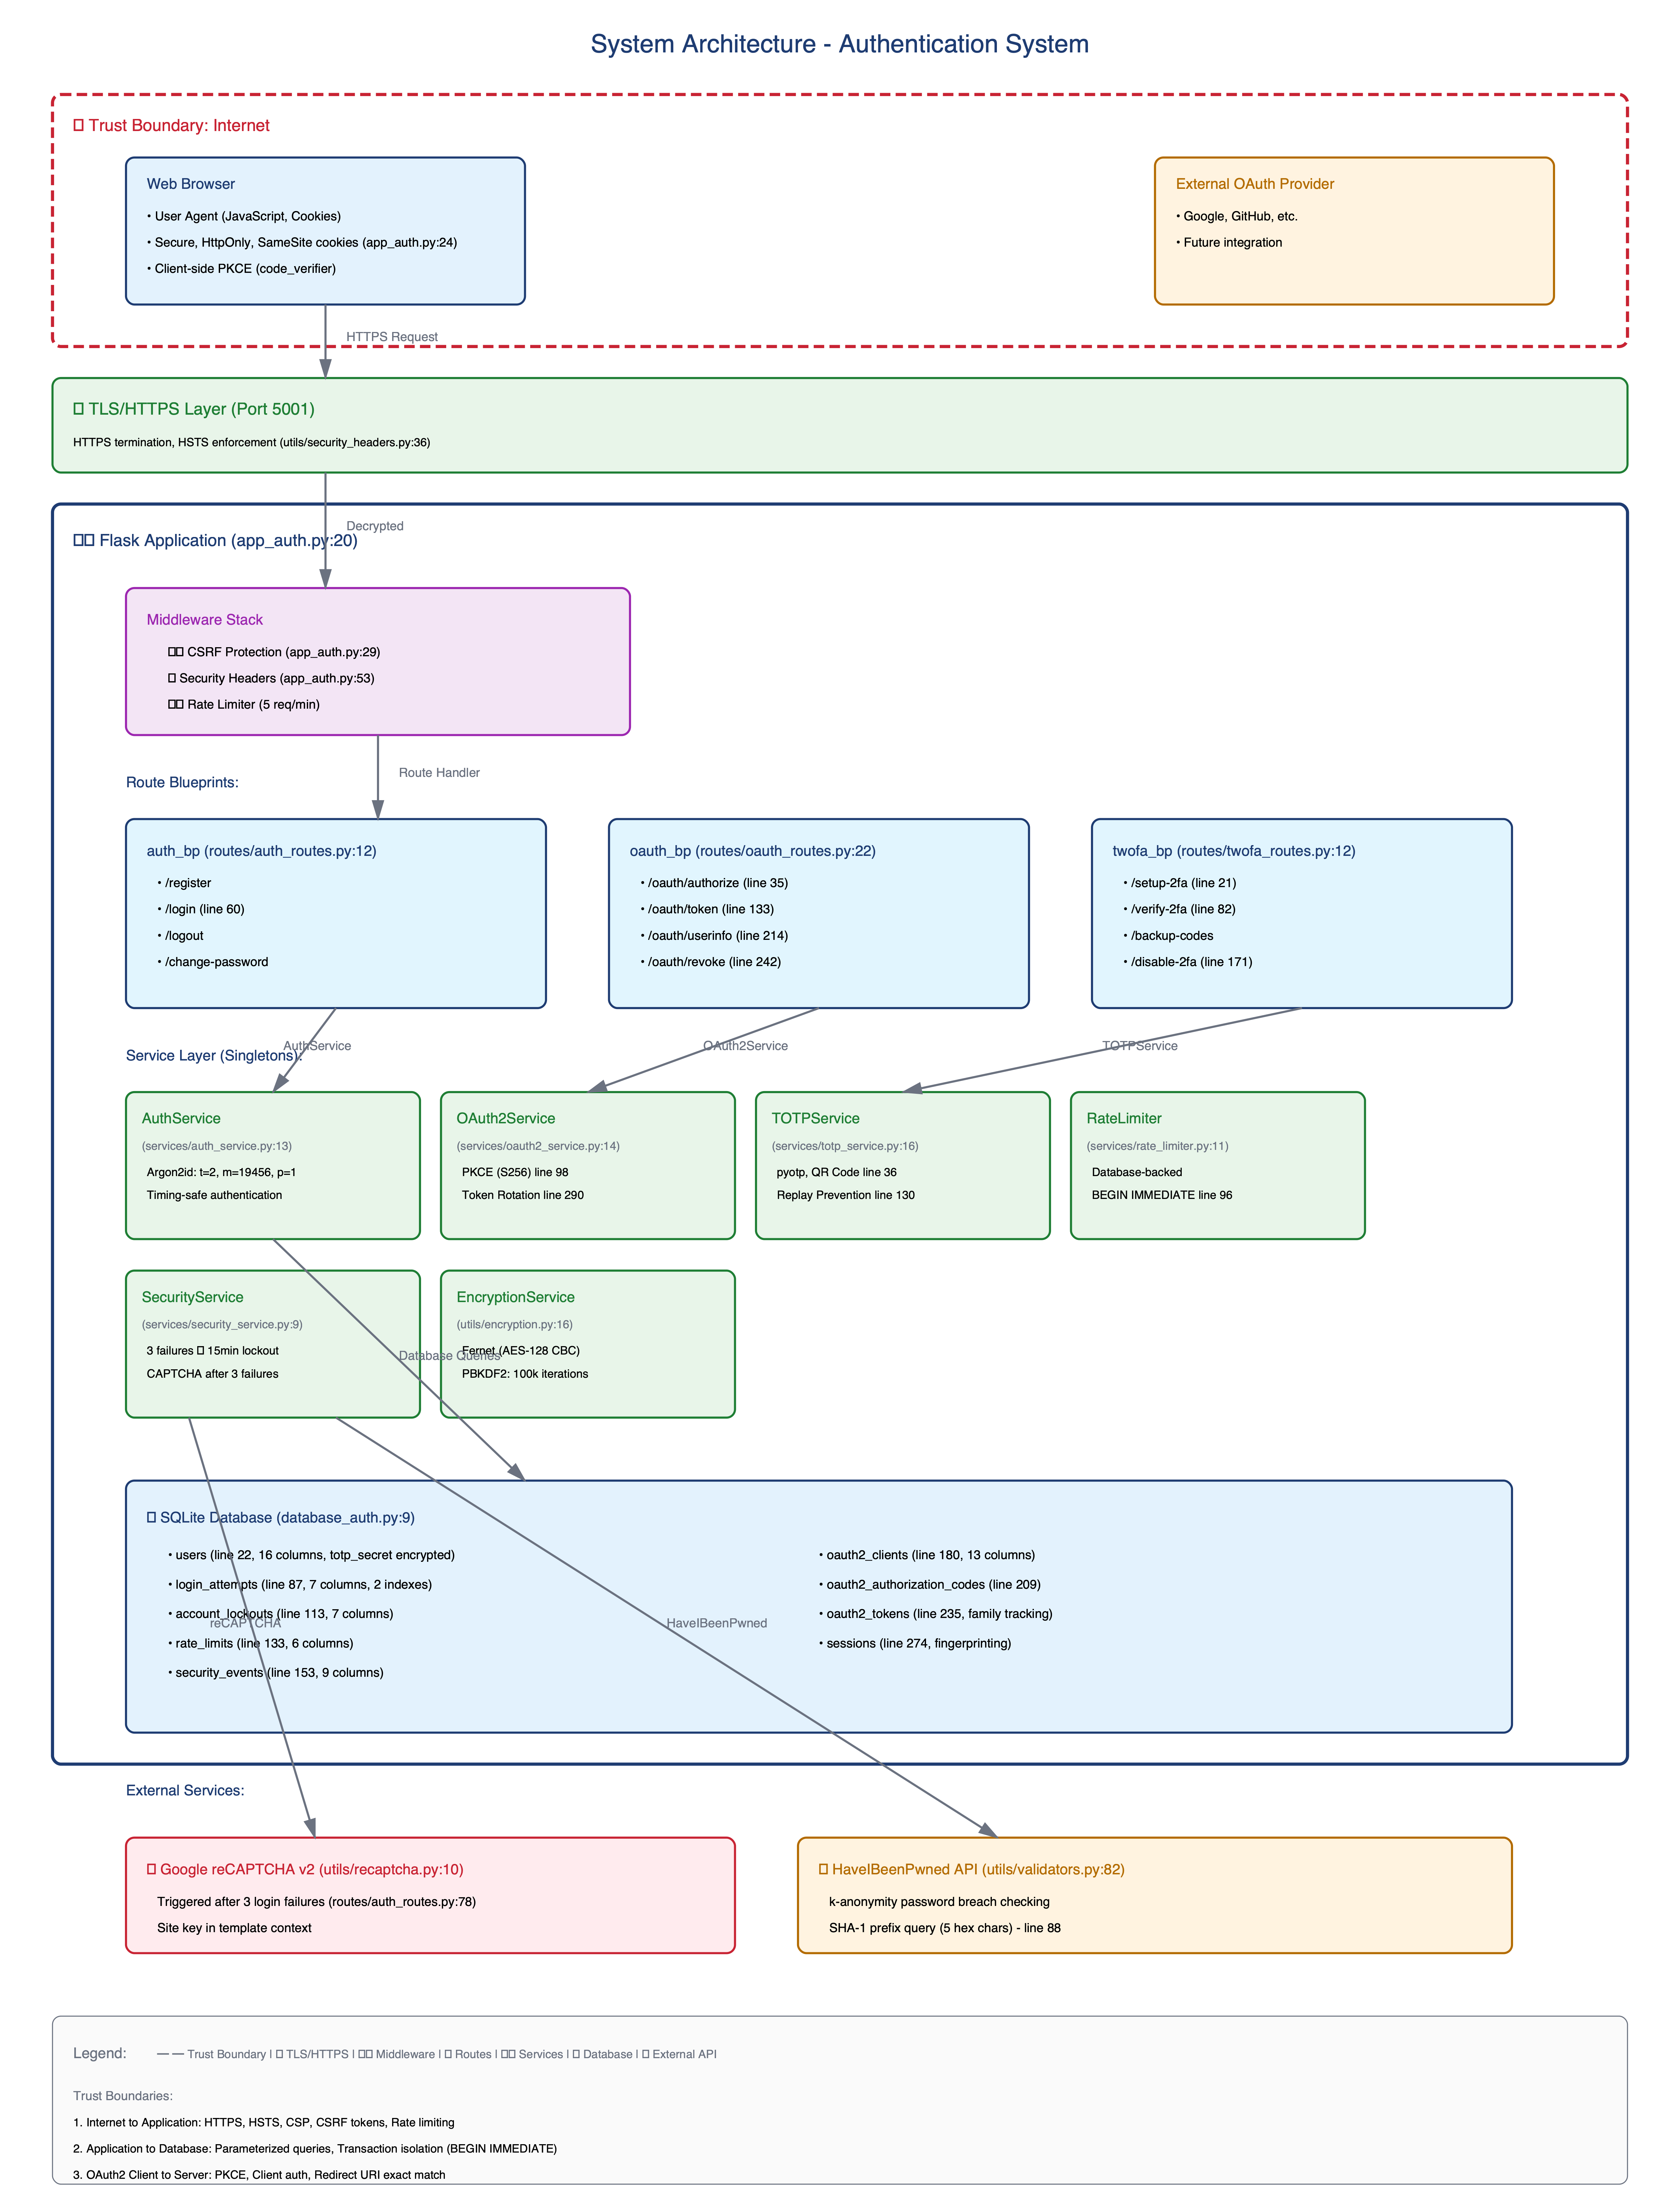
\includegraphics[width=\textwidth]{diagrams/1_system_architecture.png}
    \caption{System Architecture with middleware stack, route blueprints, services, and external integrations}
    \label{fig:architecture}
\end{figure}

The architecture includes middleware for CSRF protection, security headers, and rate limiting. External integrations include Google reCAPTCHA for bot prevention and Have I Been Pwned API for password breach detection.

\section{Task 1: Database Integration}

\subsection{Database Schema}

We designed a SQLite database with 9 tables, 15 indexes, and 8 foreign key relationships with CASCADE delete behavior. The schema supports all required authentication features while maintaining data integrity and performance.

\begin{figure}[H]
    \centering
    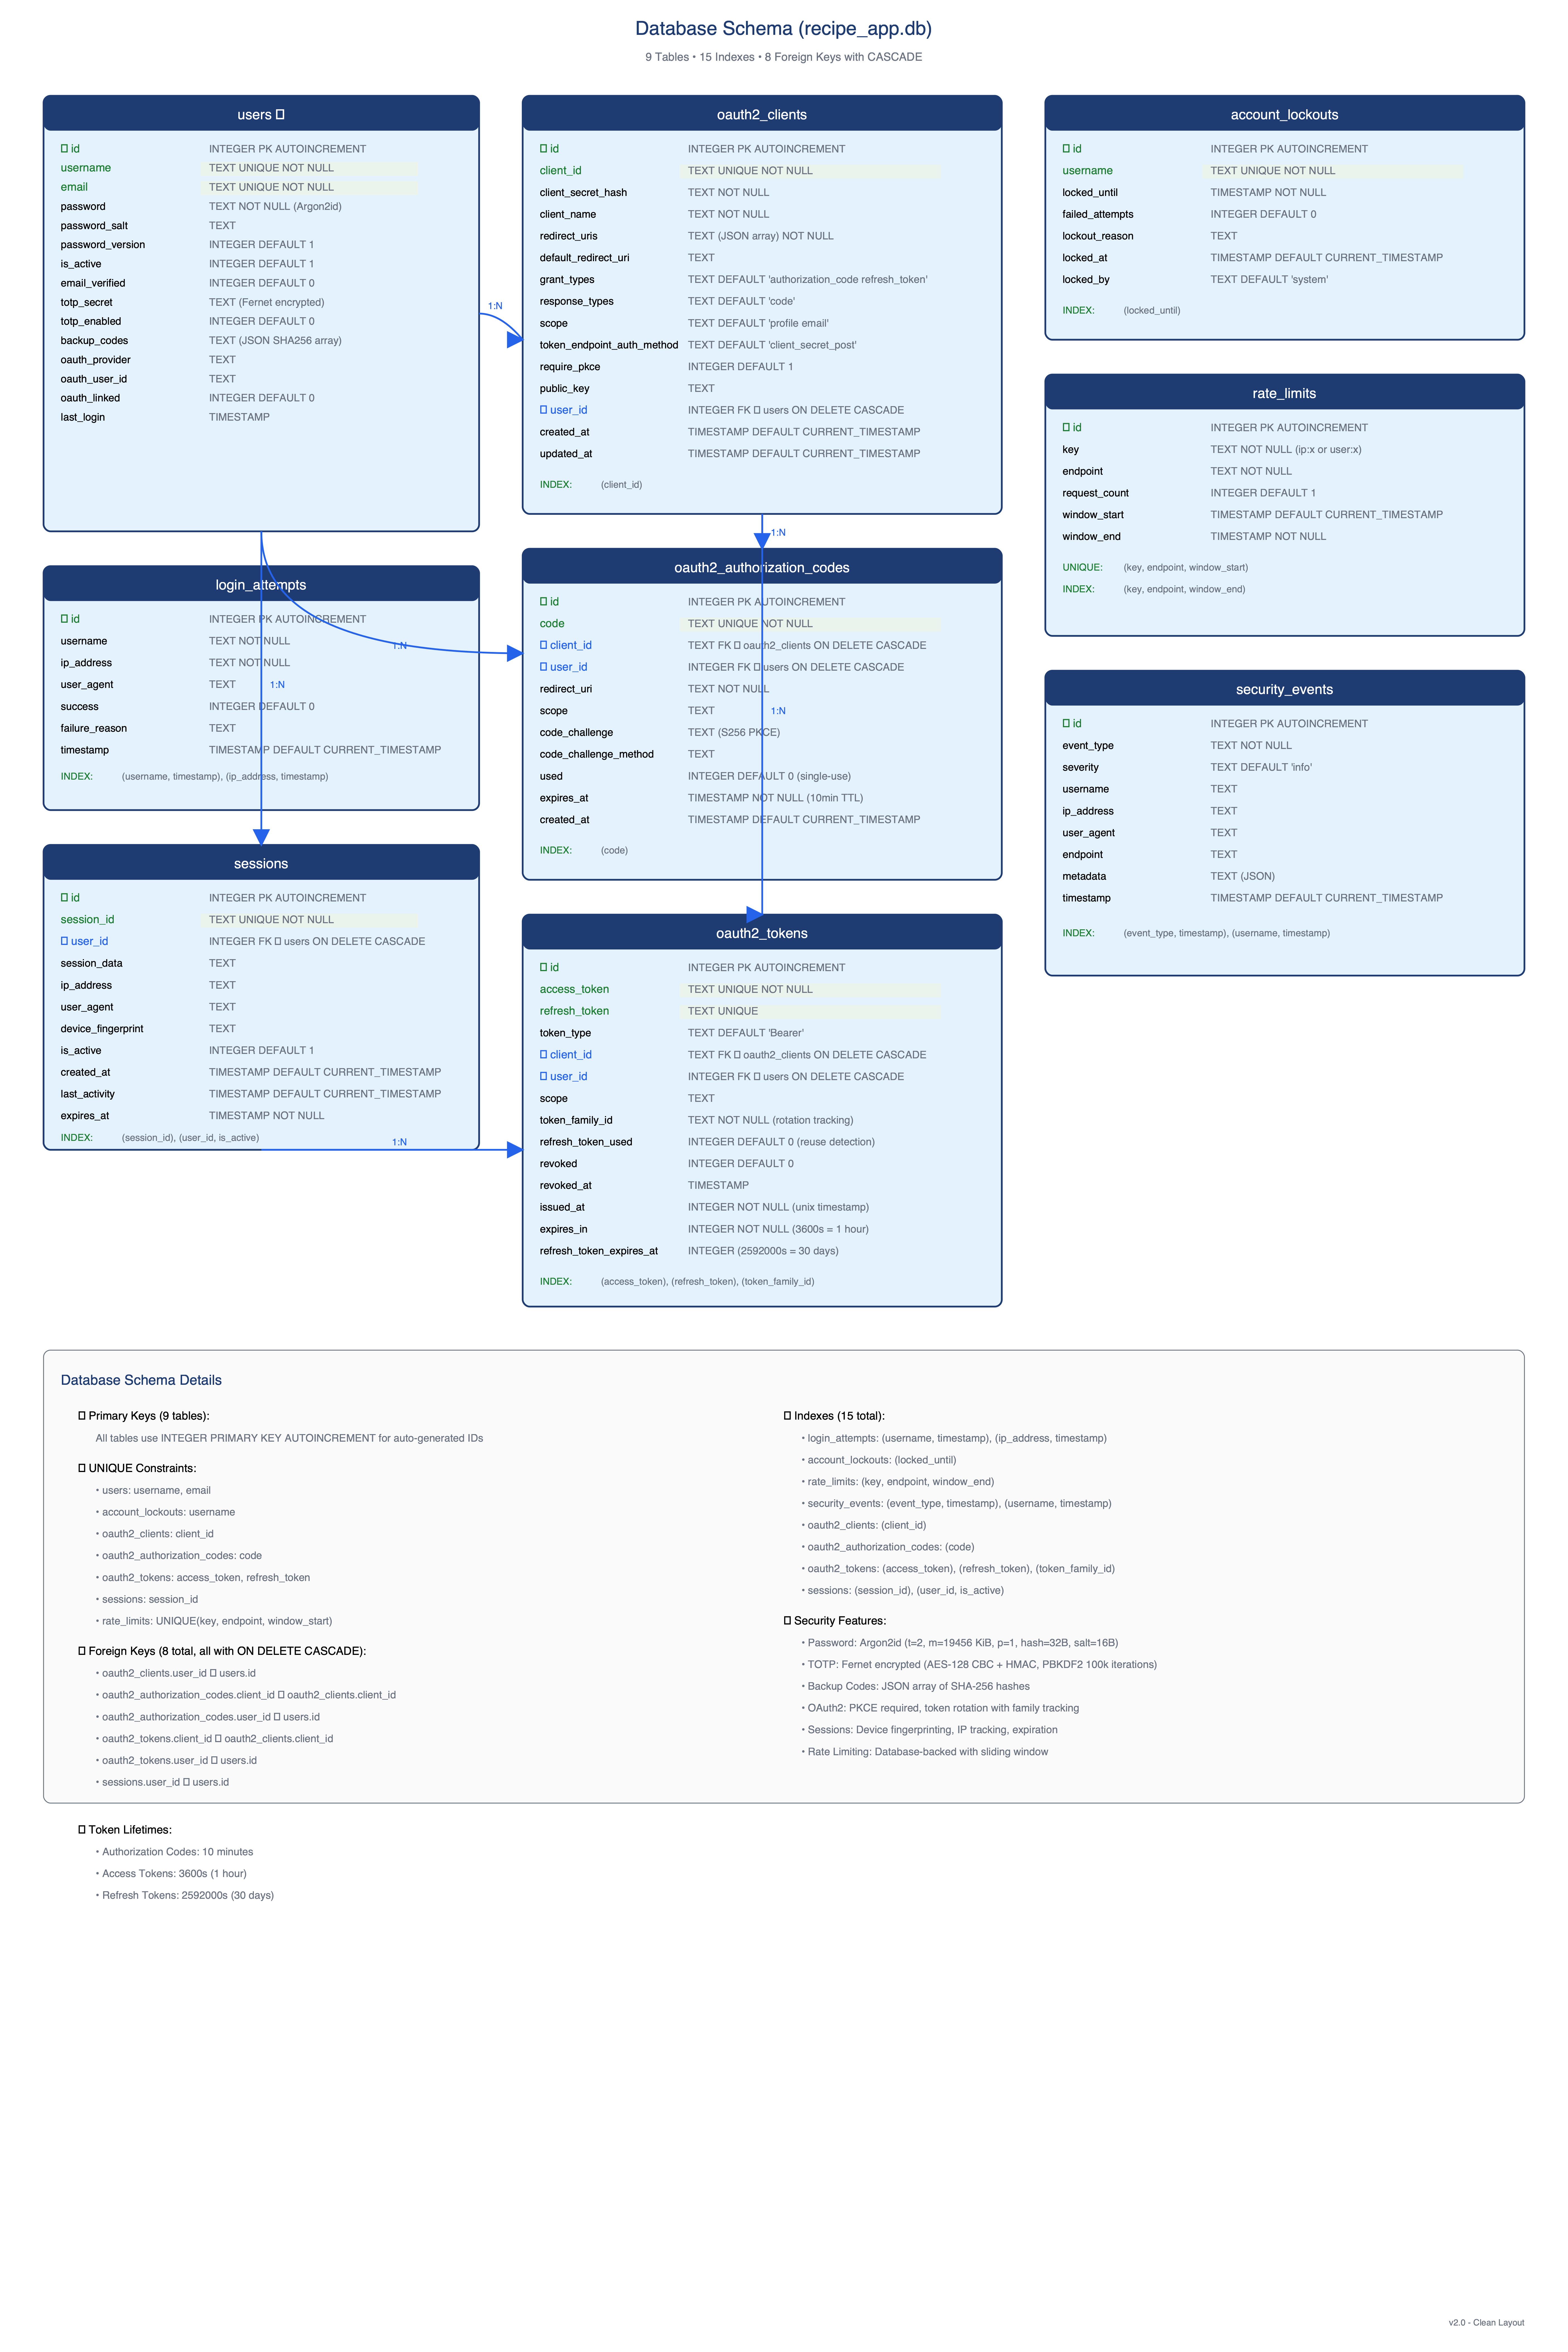
\includegraphics[width=\textwidth]{diagrams/4_database_er.png}
    \caption{Entity-Relationship Diagram showing all 9 tables with foreign key constraints}
    \label{fig:database}
\end{figure}

The database includes core authentication tables (users, login\_attempts, account\_lockouts, rate\_limits, security\_events), OAuth2 tables (oauth2\_clients, oauth2\_authorization\_codes, oauth2\_tokens), and session management. The users table has 16 columns including encrypted TOTP secrets and OAuth linking fields.

\subsection{Security Challenges and Mitigations}

\textbf{Challenge 1: SQL Injection}

Direct string concatenation allows attackers to inject malicious SQL. We prevent this using parameterized queries exclusively:

\begin{lstlisting}[language=Python]
# SECURE: Parameterized query
cursor.execute('SELECT * FROM users WHERE username = ?', (username,))
\end{lstlisting}

\textbf{Challenge 2: Race Conditions}

Multiple concurrent requests could create TOCTOU vulnerabilities. We use \texttt{BEGIN IMMEDIATE} transactions to acquire write locks immediately at 4 critical locations: authorization code validation, refresh token rotation, account lockout application, and rate limit recording.

\textbf{Challenge 3: Sensitive Data Exposure}

Sensitive data is protected with multiple encryption methods:
\begin{itemize}
    \item Passwords: Argon2id (memory-hard, GPU-resistant)
    \item TOTP secrets: Fernet encryption (AES-128 CBC + HMAC)
    \item Backup codes: SHA-256 hashing
    \item OAuth secrets: bcrypt hashing
\end{itemize}

\section{Task 2: Basic User Authentication}

\subsection{Password Hashing with Argon2id}

We use Argon2id with OWASP-recommended parameters. Argon2id won the Password Hashing Competition (2015) and is memory-hard, preventing GPU/ASIC acceleration.

\begin{lstlisting}[language=Python]
self.hasher = PasswordHasher(
    time_cost=2,         # 2 iterations
    memory_cost=19456,   # 19 MiB
    parallelism=1,
    hash_len=32,
    salt_len=16          # Auto-generated
)
\end{lstlisting}

\subsection{HIBP Breach Detection}

We integrate with Have I Been Pwned using the k-anonymity model. Only the first 5 characters of the SHA-1 hash are sent to HIBP, protecting user privacy:

\begin{lstlisting}[language=Python]
sha1 = hashlib.sha1(password.encode()).hexdigest().upper()
prefix, suffix = sha1[:5], sha1[5:]

response = requests.get(
    f'https://api.pwnedpasswords.com/range/{prefix}'
)

# Check if full hash appears in breached passwords
for line in response.text.splitlines():
    hash_suffix, count = line.split(':')
    if hash_suffix == suffix:
        return True, int(count)  # Breached!
\end{lstlisting}

\begin{figure}[H]
    \centering
    \fbox{\parbox{0.85\textwidth}{
        \centering
        \vspace{0.4cm}
        \textbf{SCREENSHOT PLACEHOLDER}\\[0.2cm]
        \textit{Registration page with HIBP breach detection}\\[0.1cm]
        \small{1. Go to http://127.0.0.1:5001/register}\\
        \small{2. Try password: "password123"}\\
        \small{3. Screenshot error: "Password found in X data breaches!"}\\
        \vspace{0.4cm}
    }}
    \caption{Registration page showing password breach detection}
    \label{fig:hibp}
\end{figure}

\subsection{Security Challenges and Mitigations}

\textbf{Challenge 1: Timing Attacks}

Attackers can determine if a username exists by measuring response times.

\textbf{Mitigation}: We perform dummy hash operations when usernames don't exist, ensuring constant-time responses regardless of username validity.

\textbf{Challenge 2: Session Fixation}

Attackers could set a victim's session ID before authentication.

\textbf{Mitigation}: Session regeneration at two critical points: after password authentication and after 2FA verification.

\section{Task 3: Protection Against Brute Force Attacks}

\subsection{Three-Layer Defense}

We implement rate limiting, account lockout, and CAPTCHA challenges as complementary defense layers. Figure \ref{fig:brute_force} shows the complete protection flow.

\begin{figure}[H]
    \centering
    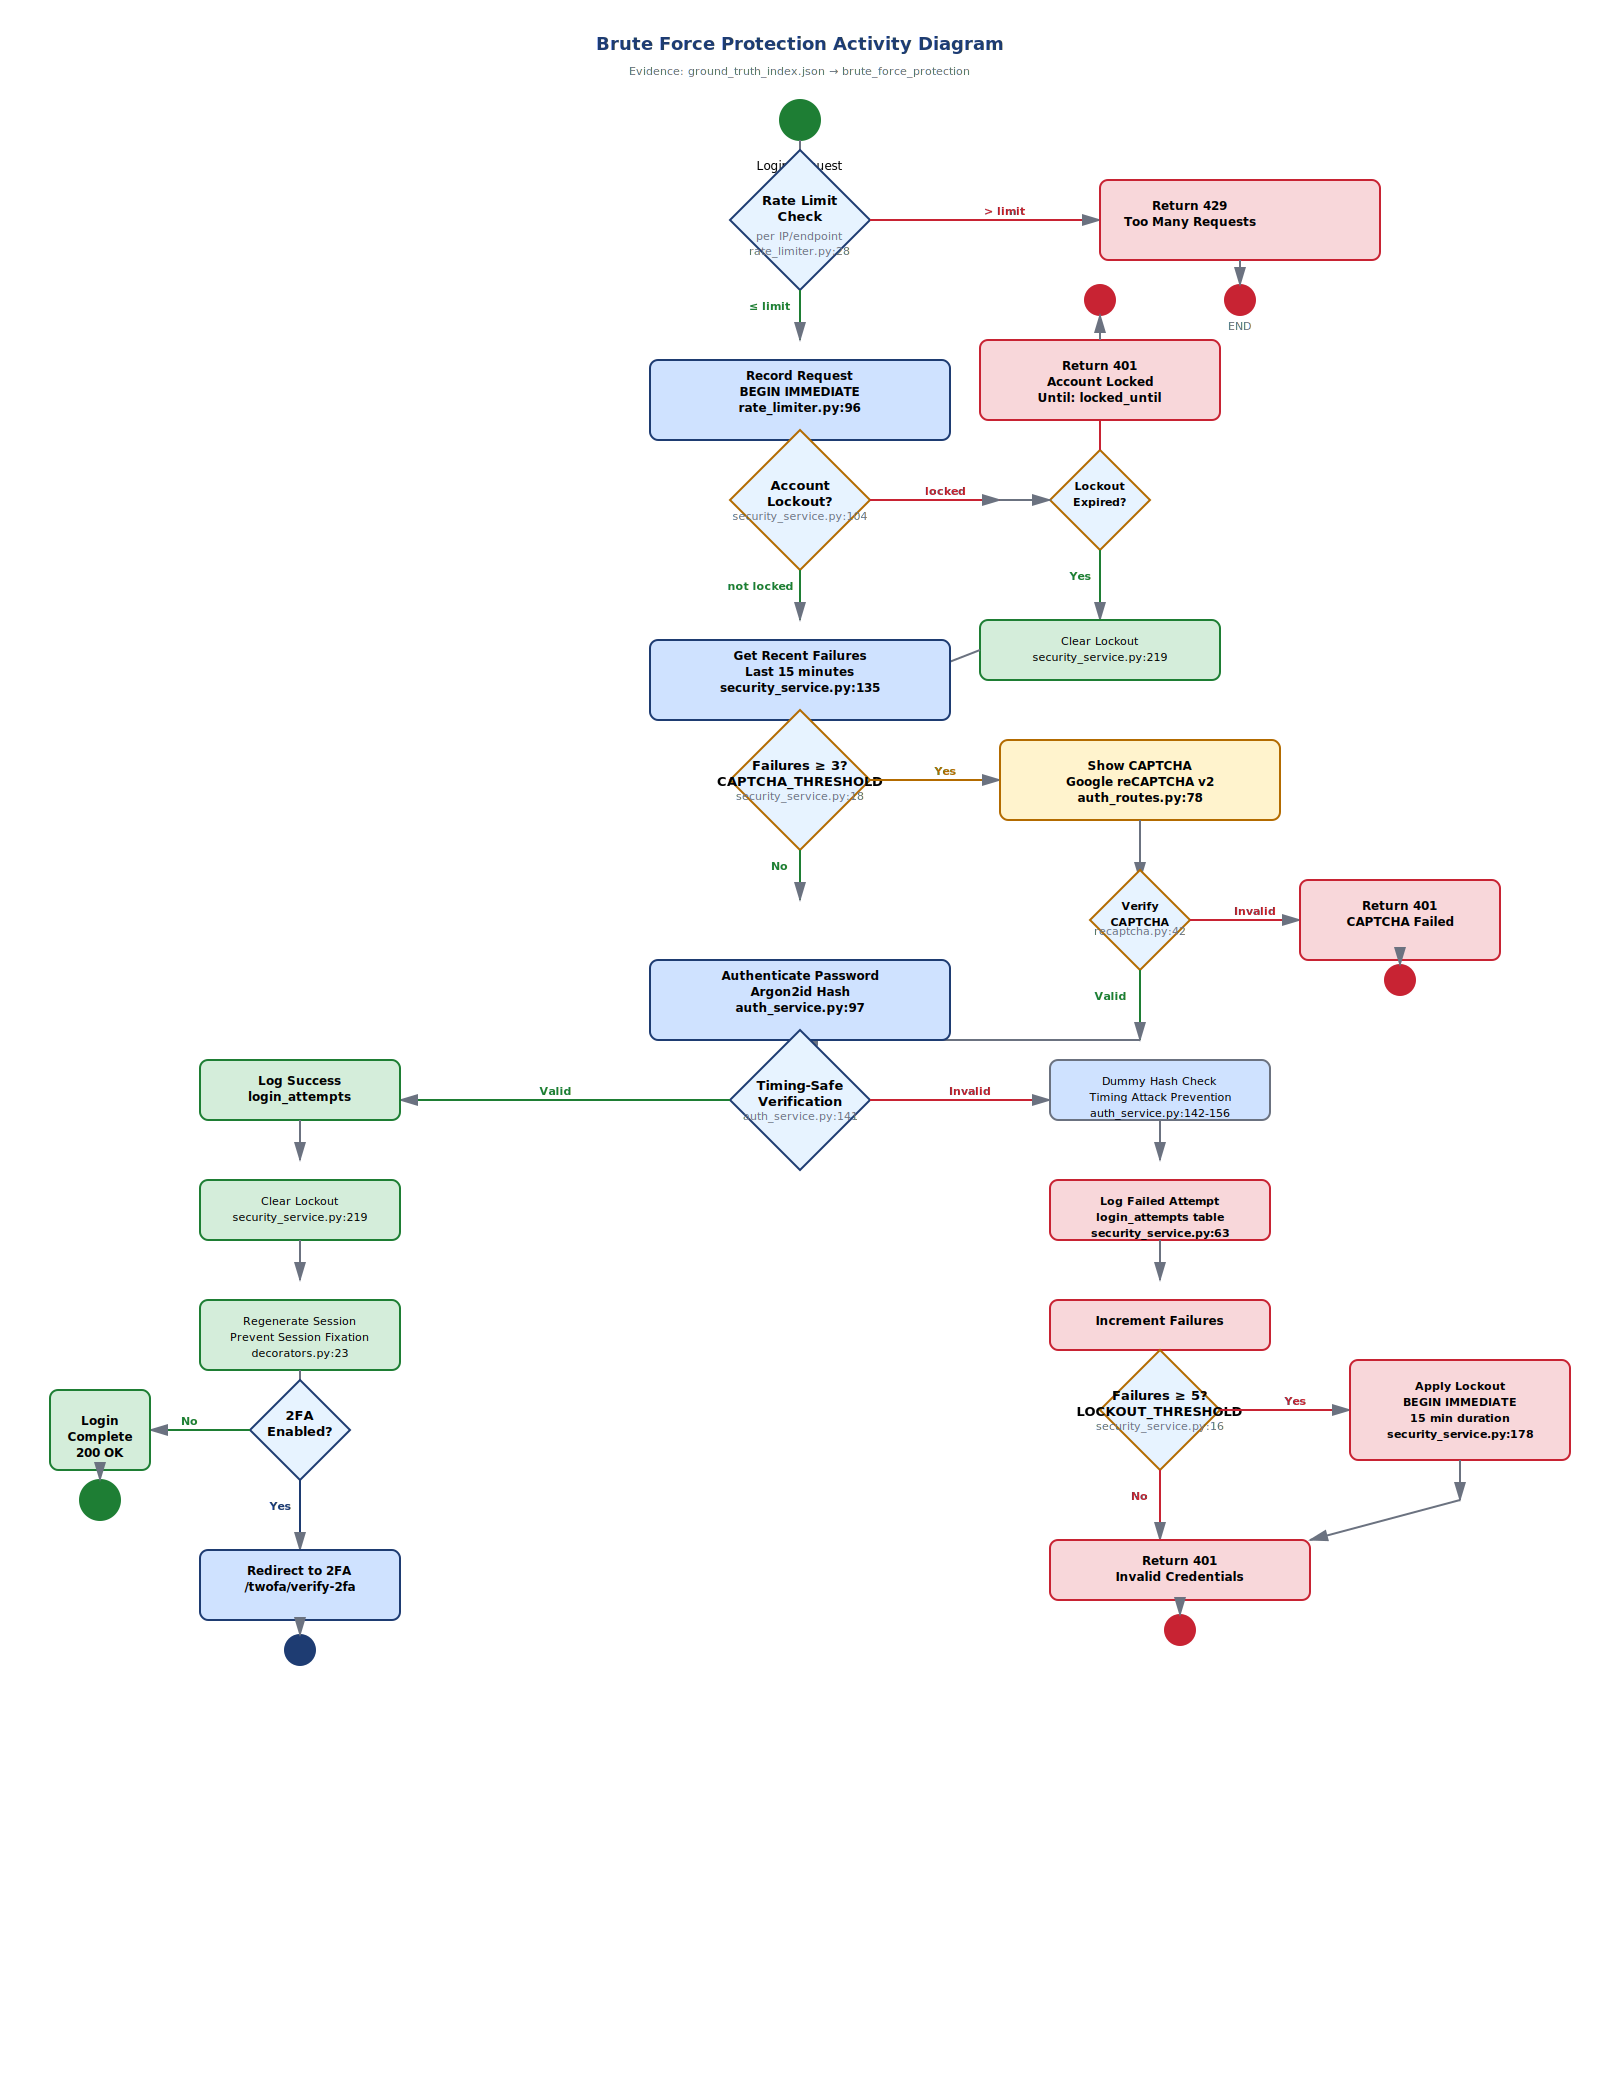
\includegraphics[width=\textwidth]{diagrams/6_brute_force_activity.png}
    \caption{Brute Force Protection Activity Diagram showing rate limiting, lockout checks, and CAPTCHA}
    \label{fig:brute_force}
\end{figure}

\textbf{Layer 1: Rate Limiting} - Database-backed, 5 requests per minute per user, returns HTTP 429 when exceeded.

\textbf{Layer 2: Account Lockout} - After 3 failed attempts within 15 minutes, accounts are locked for 15 minutes. Figure \ref{fig:lockout_state} shows the state transitions.

\begin{figure}[H]
    \centering
    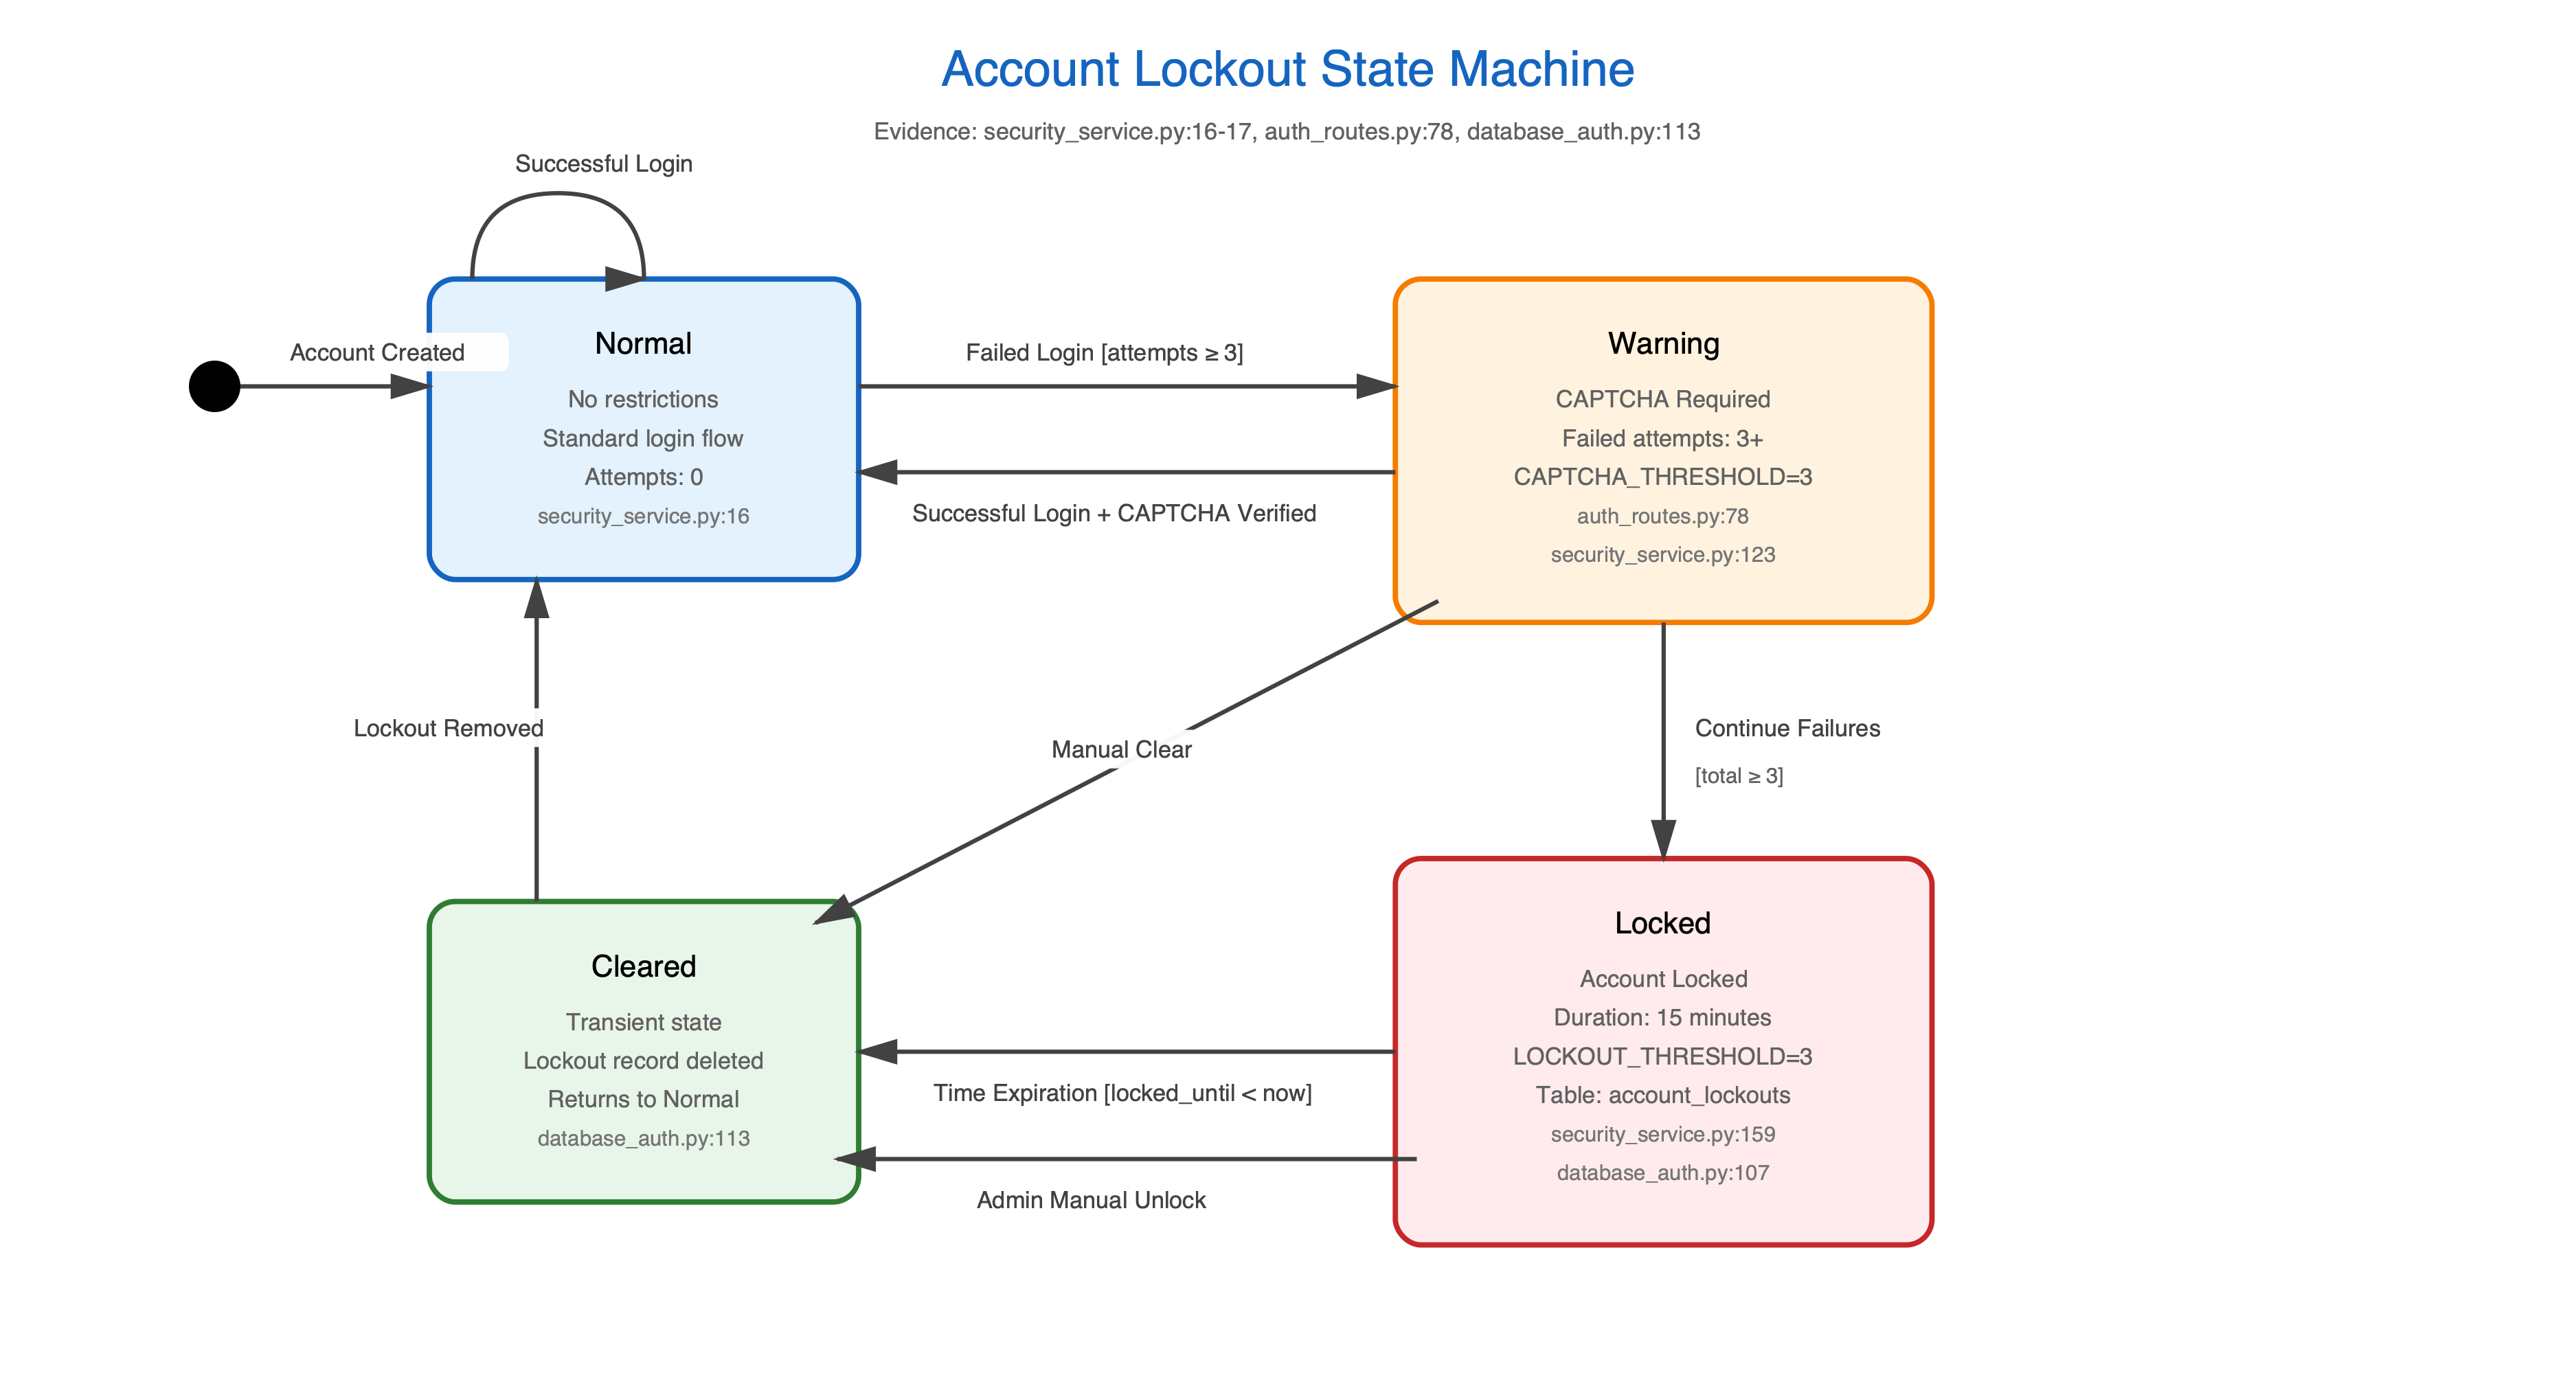
\includegraphics[width=0.65\textwidth]{diagrams/13_account_lockout_state_machine.png}
    \caption{Account Lockout State Machine}
    \label{fig:lockout_state}
\end{figure}

\textbf{Layer 3: CAPTCHA} - Google reCAPTCHA v2 required after 3 failures, prevents automated attacks.

\begin{figure}[H]
    \centering
    \fbox{\parbox{0.85\textwidth}{
        \centering
        \vspace{0.4cm}
        \textbf{SCREENSHOT PLACEHOLDER}\\[0.2cm]
        \textit{Account lockout message}\\[0.1cm]
        \small{1. Go to http://127.0.0.1:5001/login}\\
        \small{2. Fail login 3 times with wrong password}\\
        \small{3. Screenshot: "Account locked for 15 minutes"}\\
        \vspace{0.4cm}
    }}
    \caption{Account locked message after 3 failed attempts}
    \label{fig:lockout_screen}
\end{figure}

\begin{figure}[H]
    \centering
    \fbox{\parbox{0.85\textwidth}{
        \centering
        \vspace{0.4cm}
        \textbf{SCREENSHOT PLACEHOLDER}\\[0.2cm]
        \textit{Login page with CAPTCHA challenge}\\[0.1cm]
        \small{1. After lockout expires, try login again}\\
        \small{2. Screenshot showing Google reCAPTCHA checkbox}\\
        \vspace{0.4cm}
    }}
    \caption{Login page with reCAPTCHA challenge}
    \label{fig:captcha}
\end{figure}

\subsection{Security Challenges and Mitigations}

\textbf{Challenge 1: Distributed Brute Force}

Attackers using multiple IPs could bypass per-IP rate limiting.

\textbf{Mitigation}: Per-user rate limiting based on username in form data prevents distributed attacks on a single account.

\textbf{Challenge 2: Denial of Service}

Attackers could intentionally lock out legitimate users.

\textbf{Mitigation}: Short 15-minute lockout duration minimizes DoS impact while preventing brute force. Security events are logged for abuse detection.

\section{Task 4: Two-Factor Authentication}

\subsection{TOTP Implementation}

We implement Time-based One-Time Passwords (RFC 6238) using the pyotp library. Users scan a QR code with Google Authenticator or similar apps. The complete 2FA flow is shown in Figure \ref{fig:2fa_flow}.

\begin{figure}[H]
    \centering
    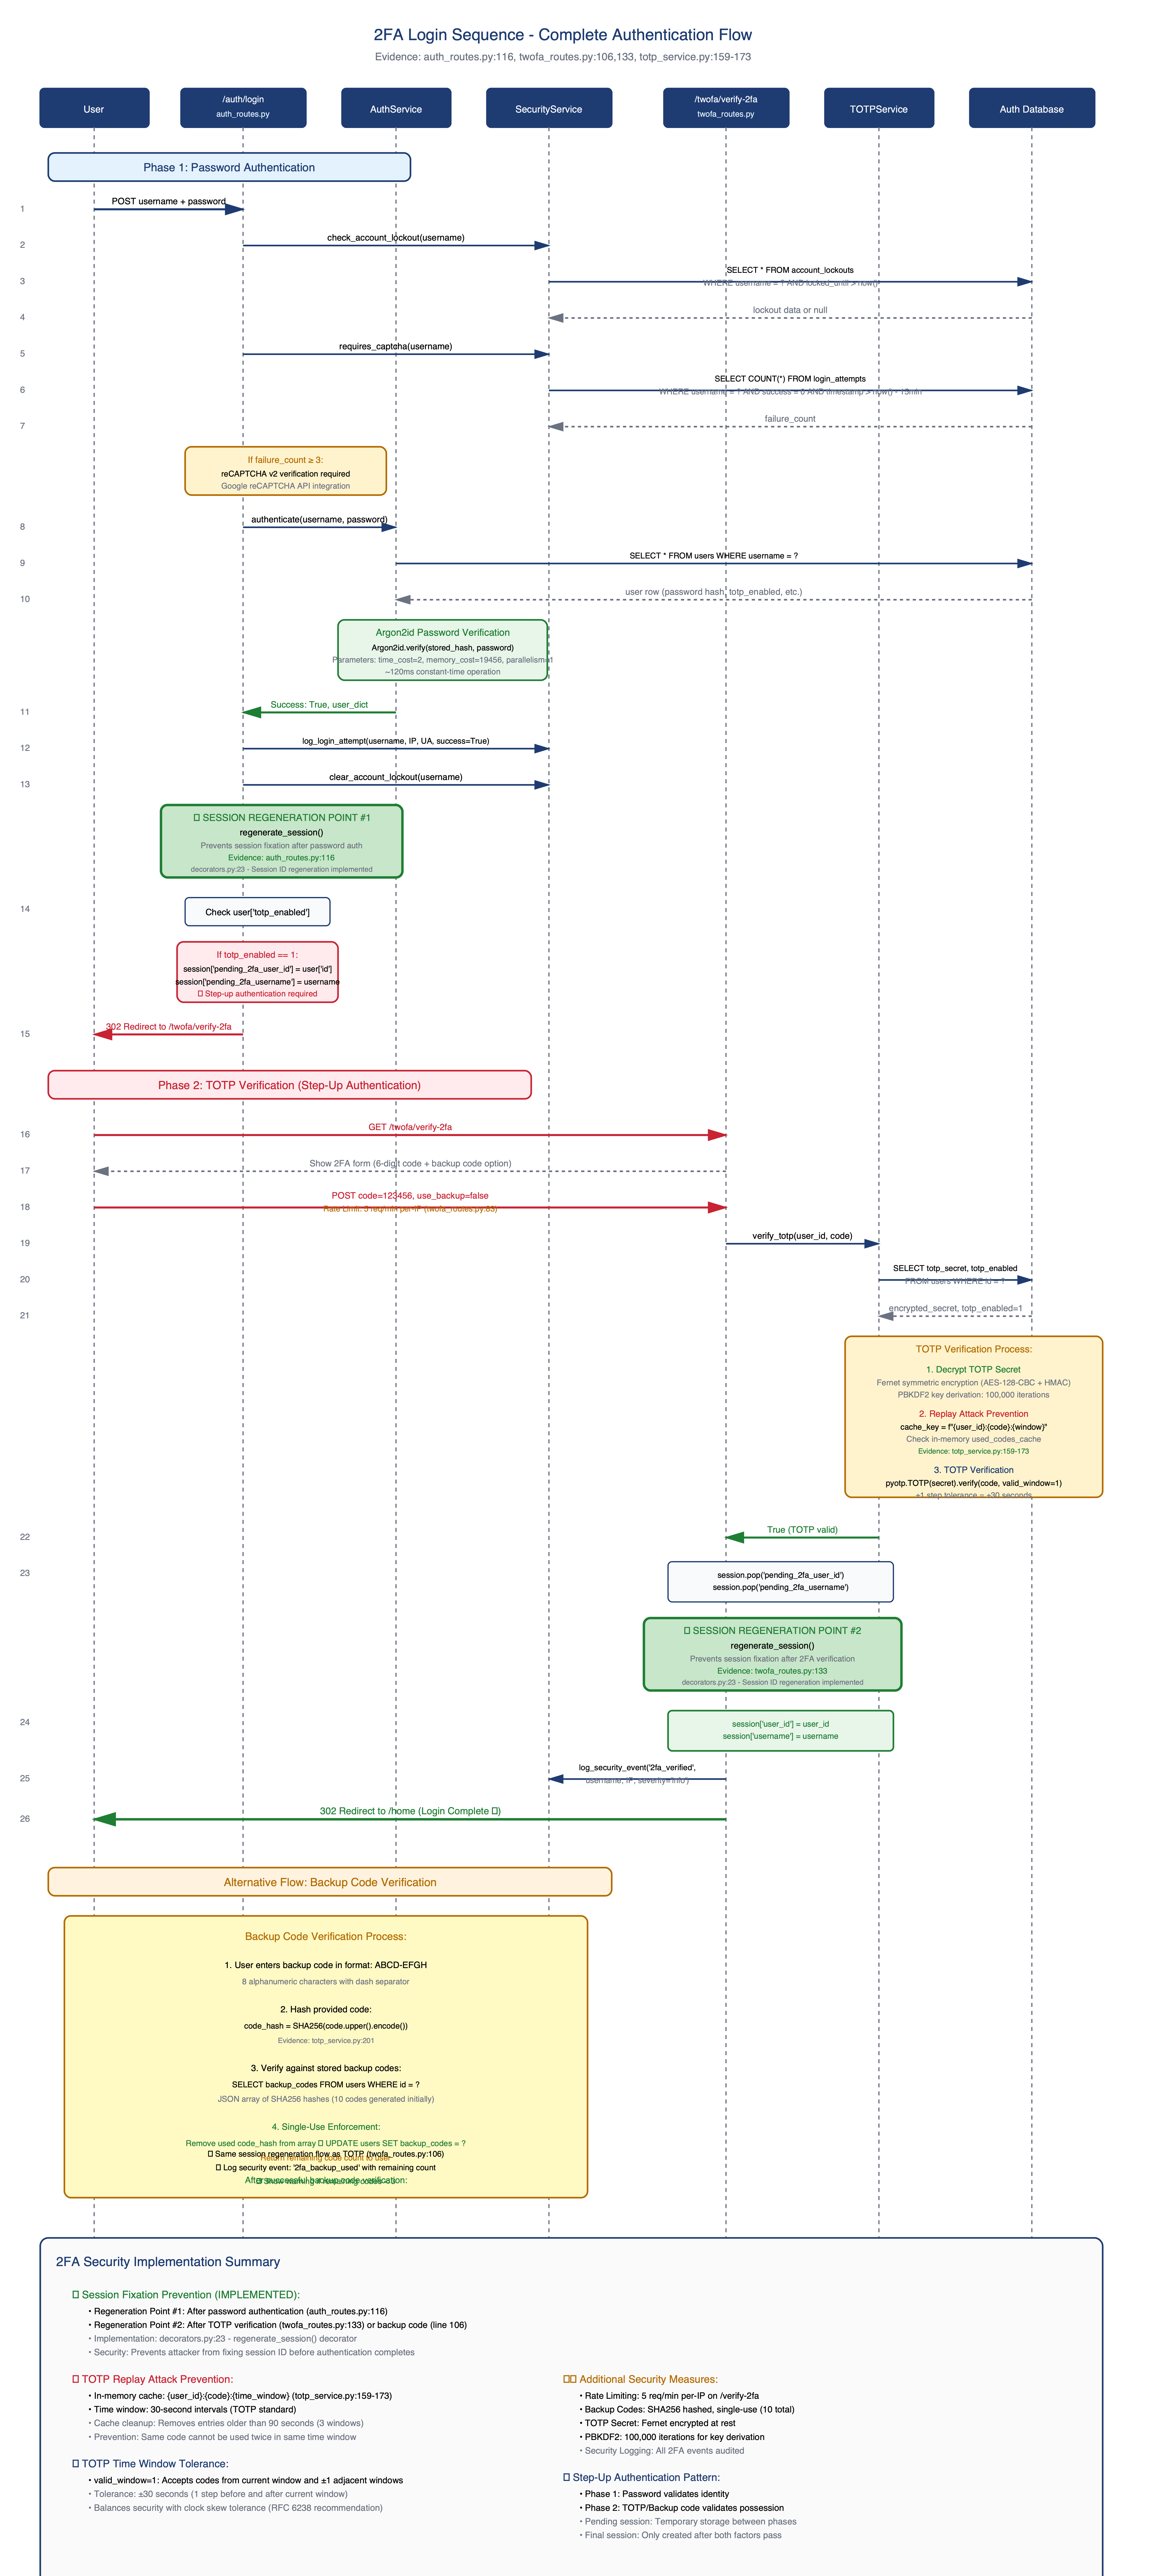
\includegraphics[width=\textwidth]{diagrams/5_2fa_login_sequence.png}
    \caption{Complete 2FA login sequence showing password authentication, session regeneration, and TOTP verification}
    \label{fig:2fa_flow}
\end{figure}

\subsection{Setup and Verification}

During setup, a random secret is generated and displayed as a QR code. Users verify by entering a TOTP code from their authenticator app. Upon successful verification, 10 backup codes are generated and displayed once.

\begin{lstlisting}[language=Python]
# Generate and verify TOTP
secret = totp_service.generate_secret()
qr_code = totp_service.generate_qr_code(secret, username)

totp = pyotp.TOTP(secret)
if totp.verify(code, valid_window=1):  # ±30 seconds
    success, backup_codes = totp_service.enable_2fa(user_id, secret)
\end{lstlisting}

\begin{figure}[H]
    \centering
    \fbox{\parbox{0.85\textwidth}{
        \centering
        \vspace{0.4cm}
        \textbf{SCREENSHOT PLACEHOLDER}\\[0.2cm]
        \textit{2FA setup page with QR code}\\[0.1cm]
        \small{1. Register new account and login}\\
        \small{2. Go to http://127.0.0.1:5001/setup-2fa}\\
        \small{3. Screenshot showing QR code and secret key}\\
        \vspace{0.4cm}
    }}
    \caption{2FA setup page with QR code for authenticator apps}
    \label{fig:2fa_setup}
\end{figure}

\begin{figure}[H]
    \centering
    \fbox{\parbox{0.85\textwidth}{
        \centering
        \vspace{0.4cm}
        \textbf{SCREENSHOT PLACEHOLDER}\\[0.2cm]
        \textit{Backup codes display}\\[0.1cm]
        \small{1. From previous step, scan QR with Google Authenticator}\\
        \small{2. Enter 6-digit code and submit}\\
        \small{3. Screenshot showing all 10 backup codes}\\
        \vspace{0.4cm}
    }}
    \caption{One-time display of 10 backup codes after 2FA setup}
    \label{fig:backup}
\end{figure}

\subsection{Replay Prevention}

TOTP codes are valid for 30 seconds. We prevent replay attacks by caching used codes:

\begin{lstlisting}[language=Python]
# Check if code already used in this time window
current_window = int(datetime.utcnow().timestamp() // 30)
cache_key = f"{user_id}:{code}:{current_window}"

if cache_key in self.used_codes_cache:
    return False, 'Code already used'

# Verify and mark as used
if totp.verify(code, valid_window=1):
    self.used_codes_cache[cache_key] = True
\end{lstlisting}

\begin{figure}[H]
    \centering
    \fbox{\parbox{0.85\textwidth}{
        \centering
        \vspace{0.4cm}
        \textbf{SCREENSHOT PLACEHOLDER}\\[0.2cm]
        \textit{2FA verification page}\\[0.1cm]
        \small{1. Logout and login again with 2FA-enabled account}\\
        \small{2. After password, screenshot TOTP code input page}\\
        \vspace{0.4cm}
    }}
    \caption{2FA verification page requesting TOTP code}
    \label{fig:2fa_verify}
\end{figure}

\subsection{Security Challenges and Mitigations}

\textbf{Challenge 1: Secret Exposure}

If the database is compromised, TOTP secrets could be stolen.

\textbf{Mitigation}: Secrets are encrypted with Fernet (AES-128) using PBKDF2 key derivation with 100,000 iterations.

\textbf{Challenge 2: Replay Attacks}

Intercepted codes could be reused within the valid time window.

\textbf{Mitigation}: In-memory cache tracks used codes per 30-second window with automatic cleanup.

\textbf{Challenge 3: Clock Skew}

Server and client clocks might not be synchronized.

\textbf{Mitigation}: \texttt{valid\_window=1} accepts codes from ±30 seconds (previous and next window).

\section{Task 5: OAuth2 Implementation}

\subsection{Authorization Code Flow with PKCE}

We implement OAuth2 Authorization Code Flow with mandatory PKCE (Proof Key for Code Exchange) following RFC 7636. PKCE prevents authorization code interception attacks.

\begin{figure}[H]
    \centering
    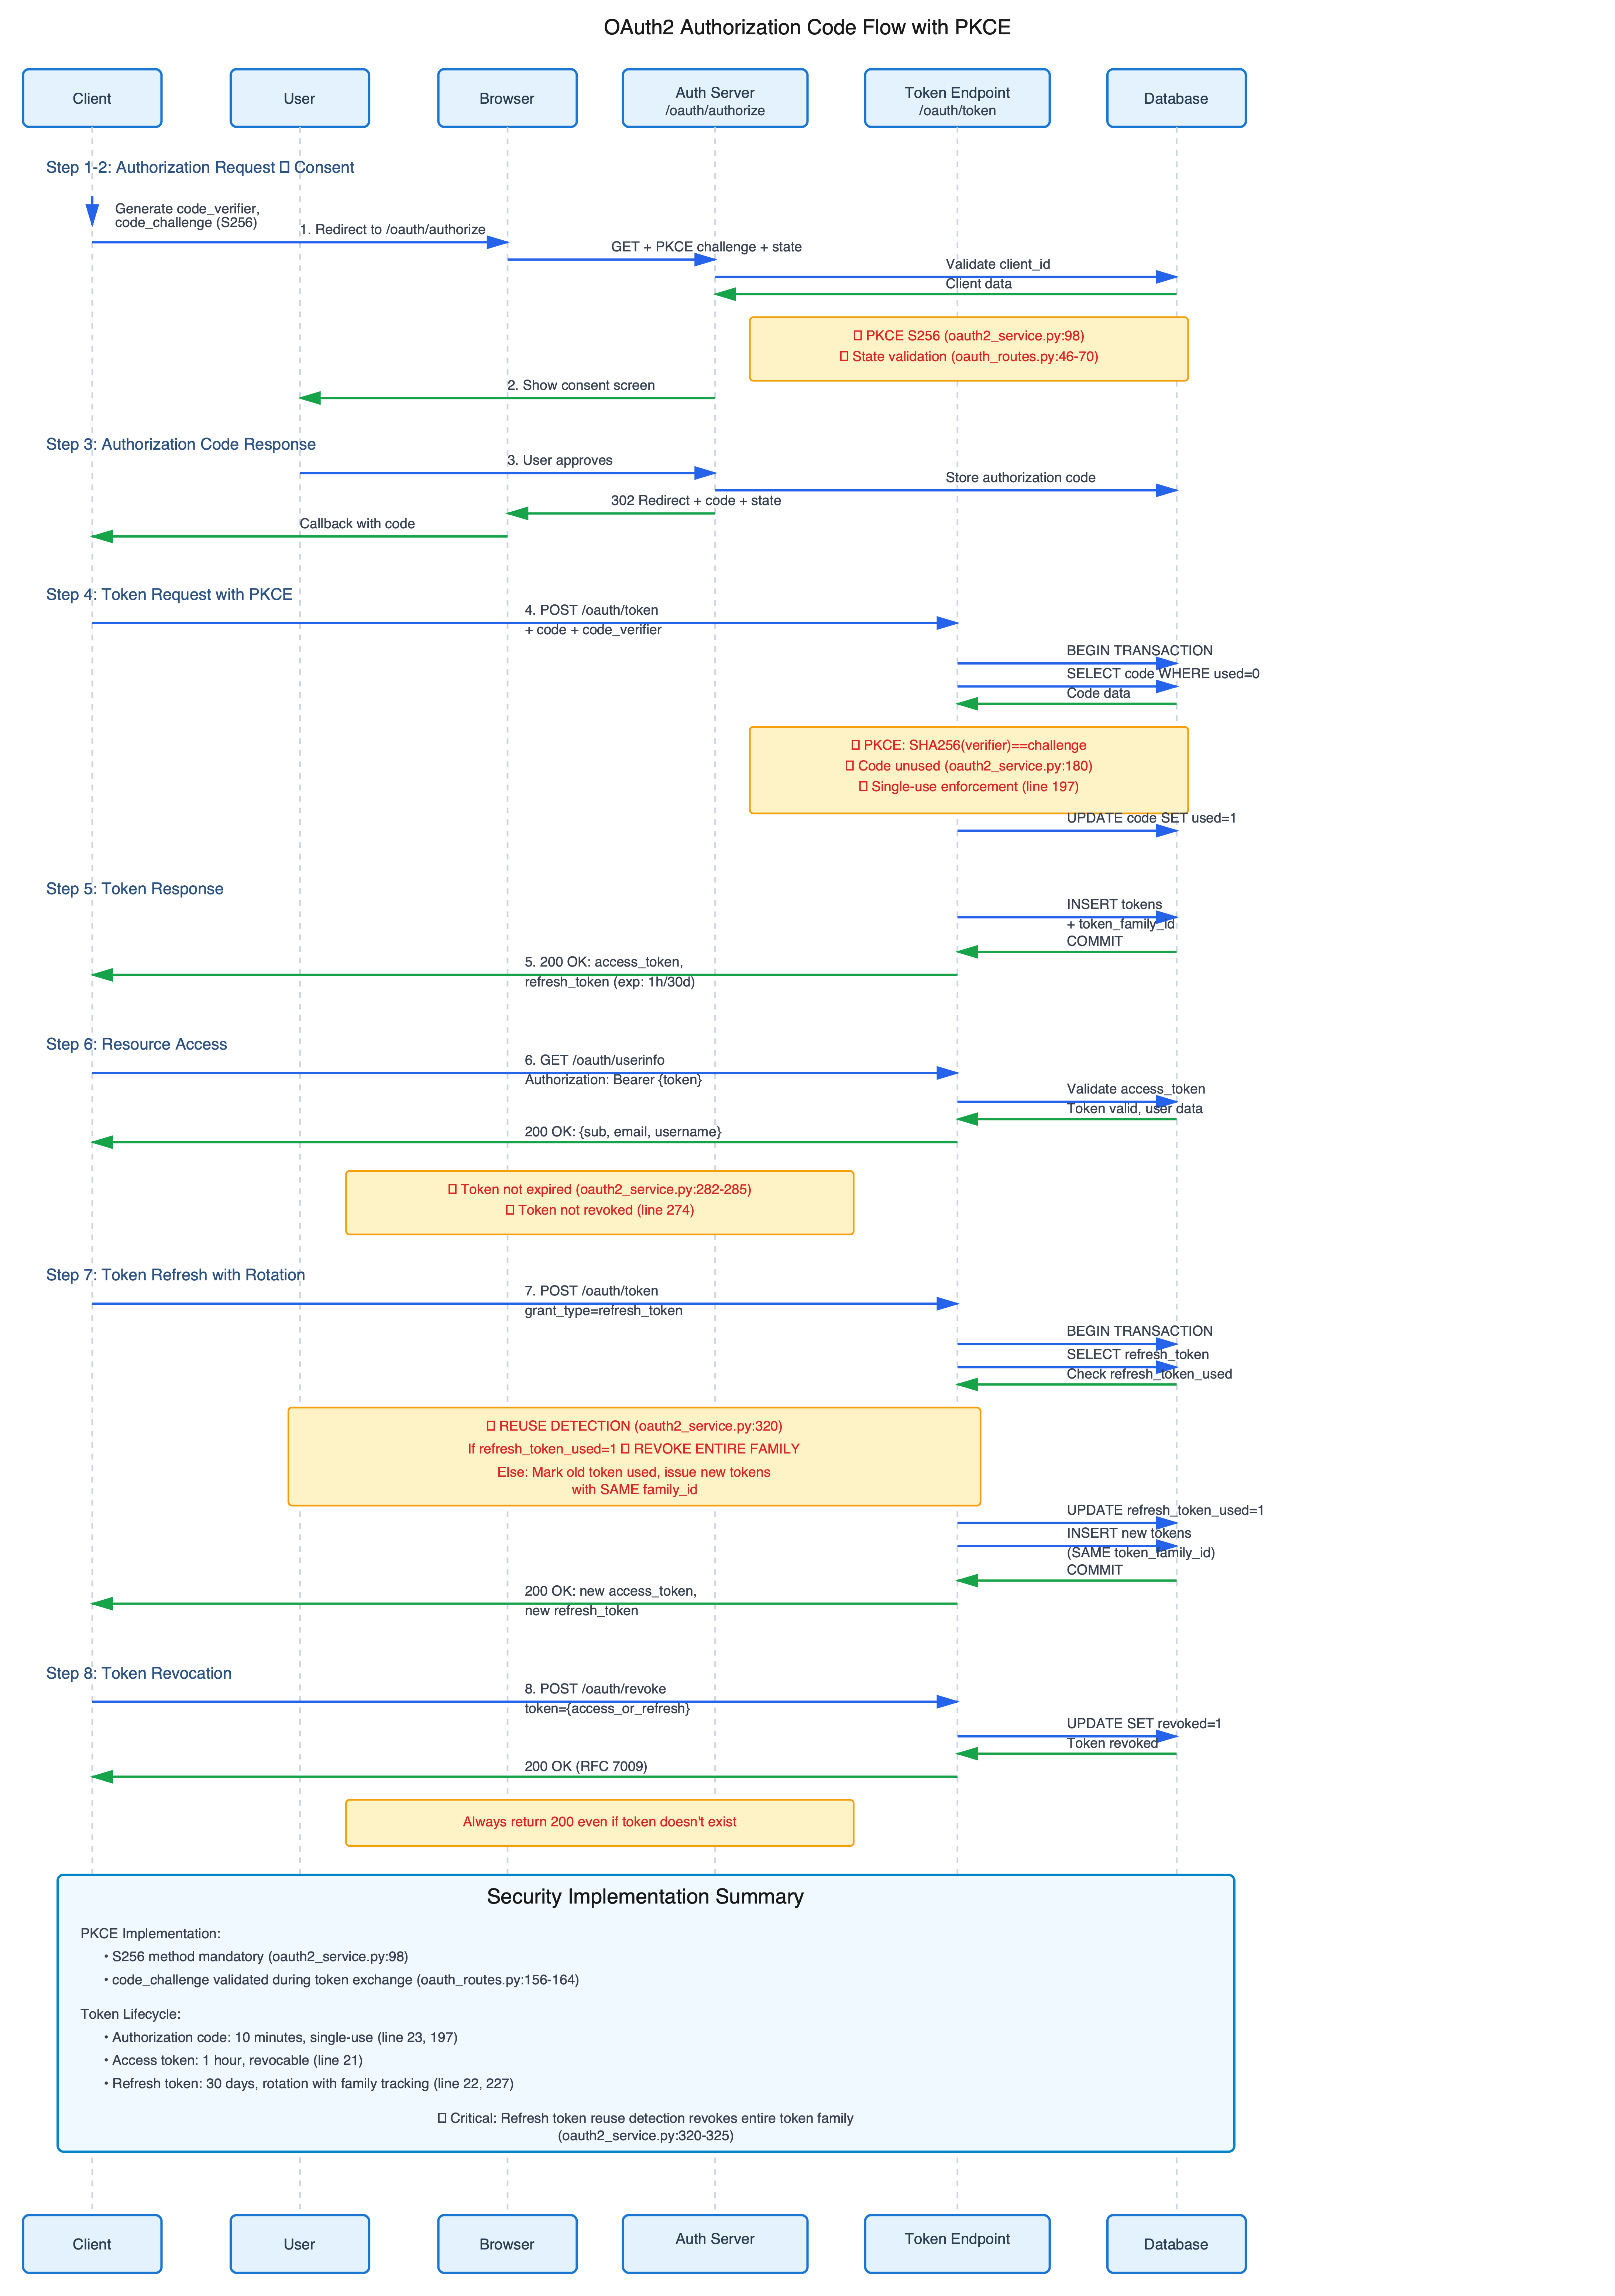
\includegraphics[width=\textwidth]{diagrams/3_oauth2_sequence.png}
    \caption{Complete OAuth2 flow with PKCE validation and token generation}
    \label{fig:oauth2}
\end{figure}

\subsection{PKCE Process}

PKCE adds security by requiring the client to prove they initiated the authorization request:

\begin{enumerate}
    \item Client generates random \texttt{code\_verifier}
    \item Client computes \texttt{code\_challenge = BASE64URL(SHA256(code\_verifier))}
    \item Authorization request includes \texttt{code\_challenge}
    \item Token exchange requires \texttt{code\_verifier}
    \item Server validates: \texttt{SHA256(code\_verifier) == code\_challenge}
\end{enumerate}

Even if the authorization code is intercepted, it's useless without the original \texttt{code\_verifier}.

\begin{lstlisting}[language=Python, caption=PKCE Validation]
def validate_pkce(self, code_verifier, code_challenge,
                  code_challenge_method='S256'):
    sha256_hash = hashlib.sha256(code_verifier.encode()).digest()
    computed = base64.urlsafe_b64encode(sha256_hash).decode().rstrip('=')
    return computed == code_challenge
\end{lstlisting}

\begin{figure}[H]
    \centering
    \fbox{\parbox{0.85\textwidth}{
        \centering
        \vspace{0.4cm}
        \textbf{SCREENSHOT PLACEHOLDER}\\[0.2cm]
        \textit{OAuth2 consent screen}\\[0.1cm]
        \small{1. Register OAuth client (use tests/test\_oauth2\_teacher.py)}\\
        \small{2. Navigate to /oauth/authorize with client\_id and code\_challenge}\\
        \small{3. Screenshot consent screen showing client name and scopes}\\
        \vspace{0.4cm}
    }}
    \caption{OAuth2 authorization consent screen}
    \label{fig:oauth_consent}
\end{figure}

\subsection{Refresh Token Rotation}

Modern OAuth2 security requires refresh token rotation to detect token theft. Figure \ref{fig:token_rotation} shows the rotation mechanism.

\begin{figure}[H]
    \centering
    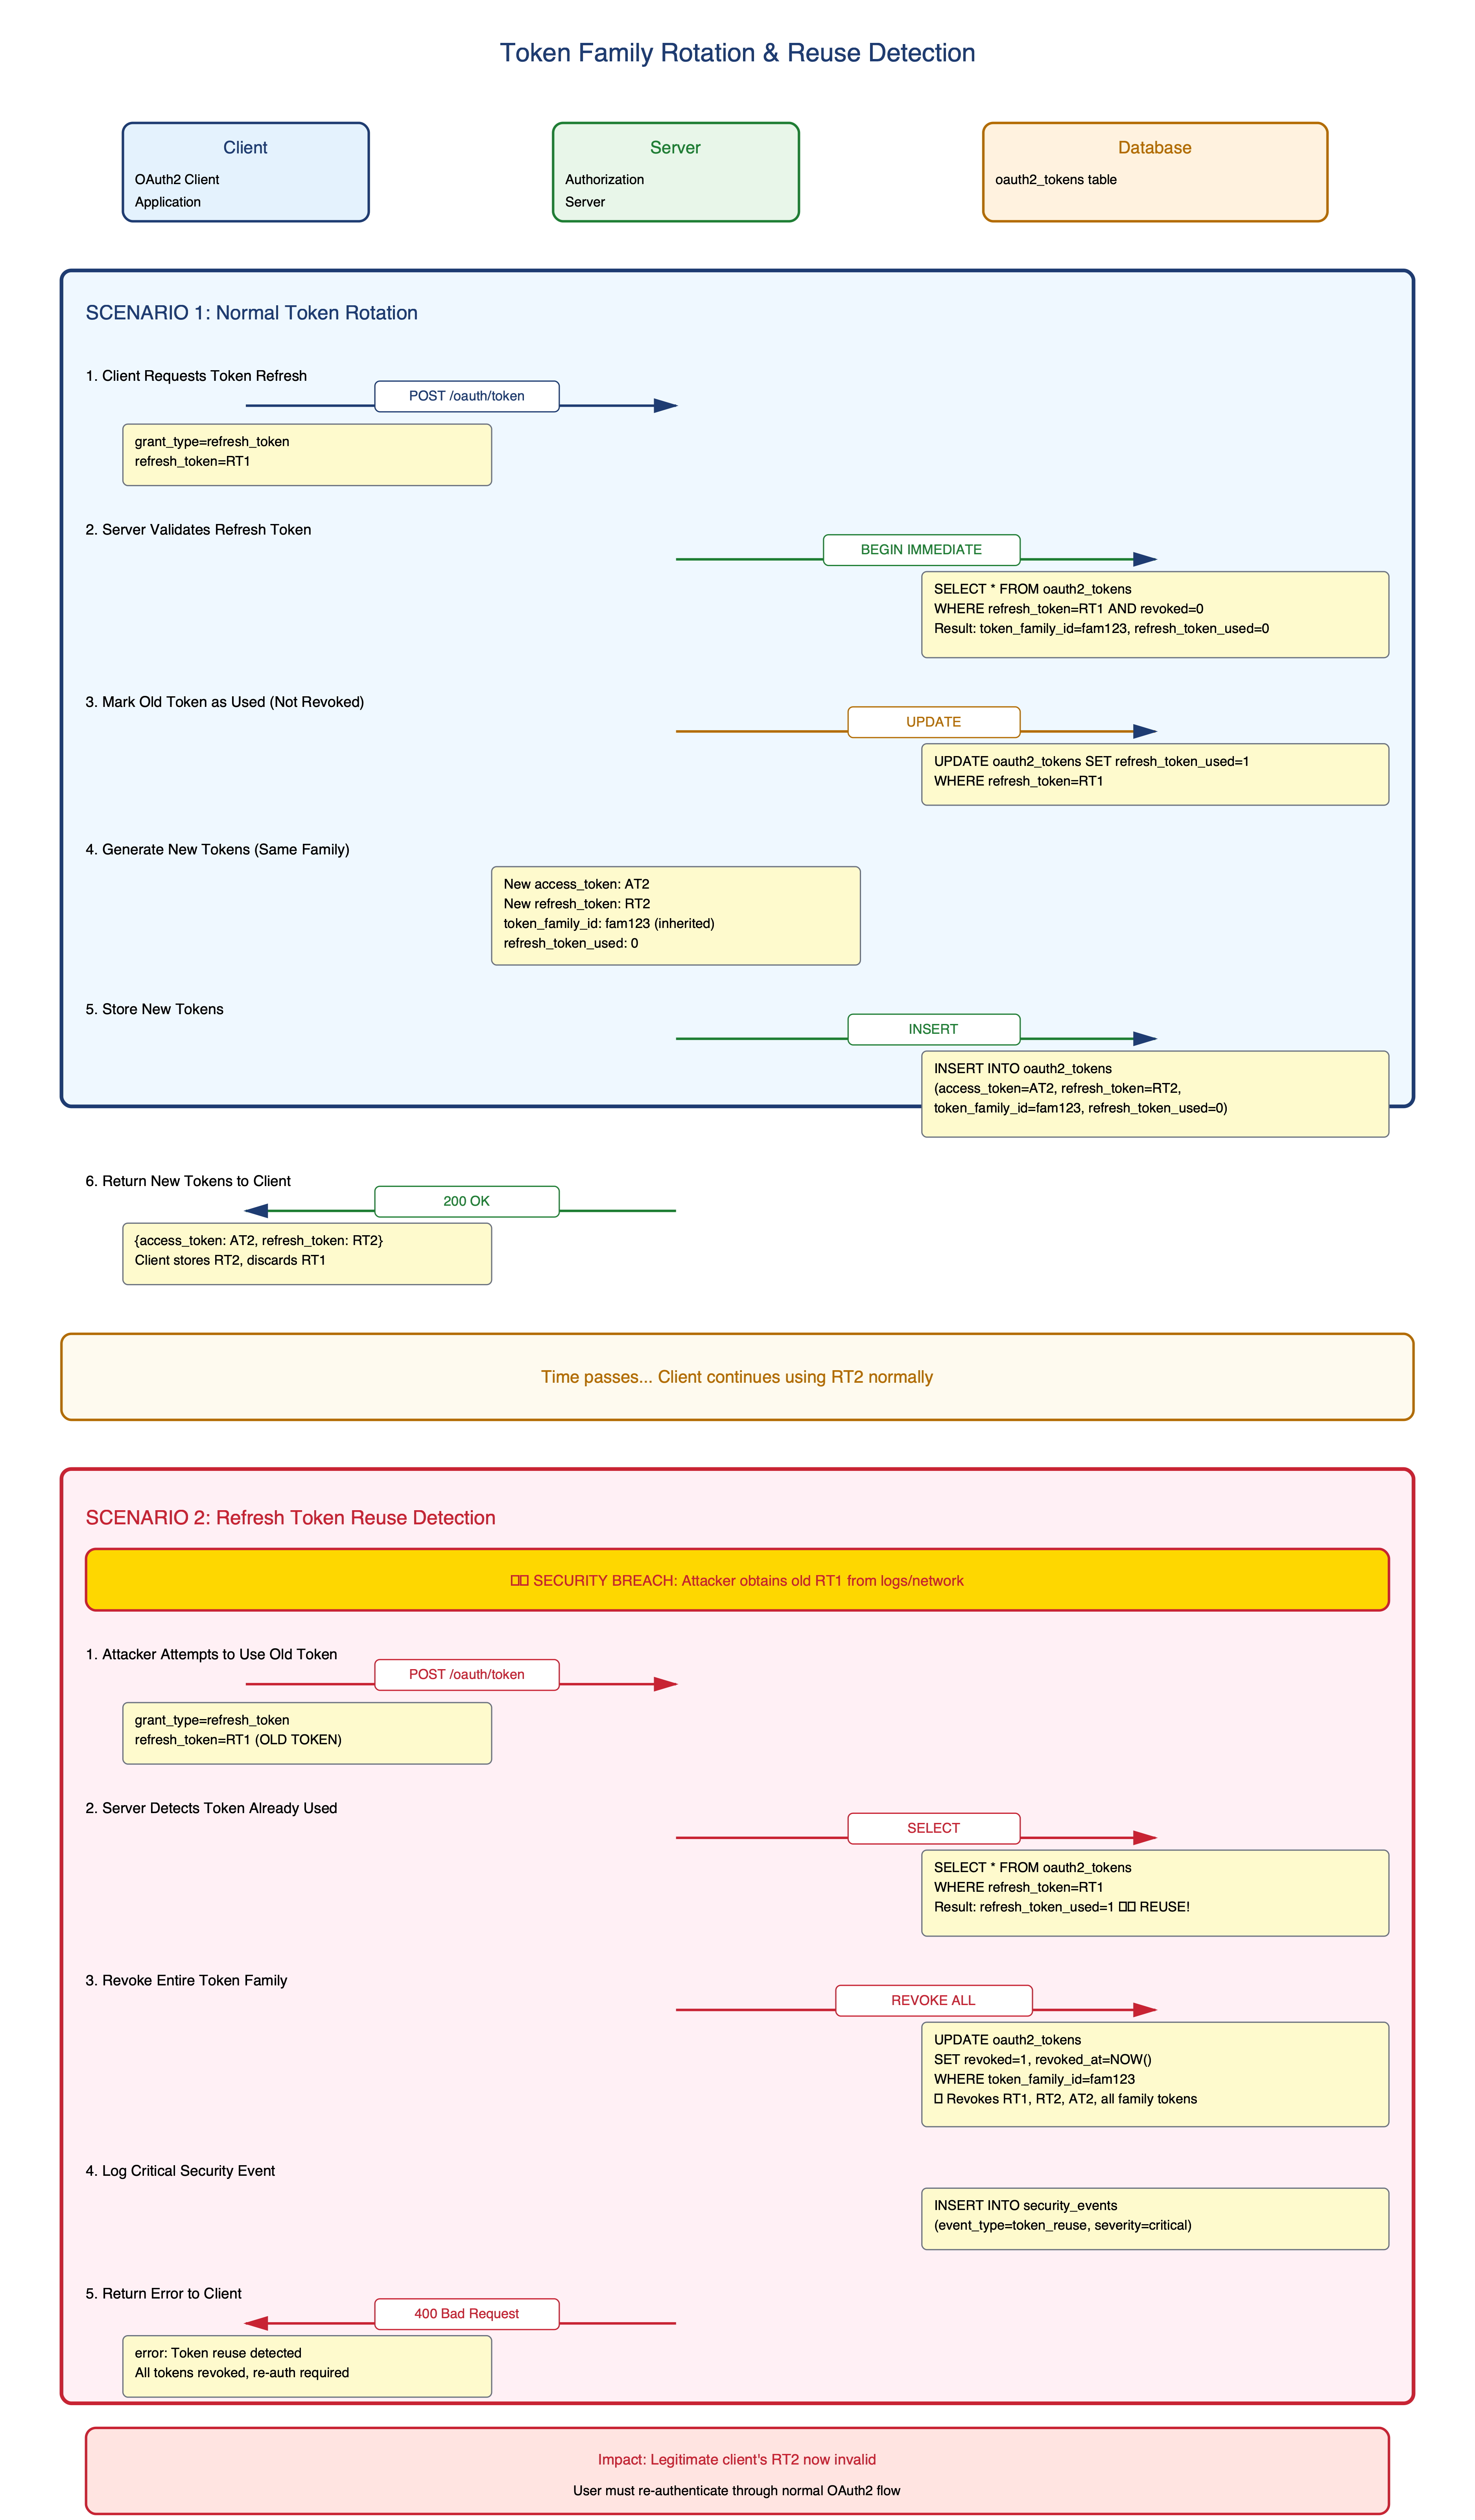
\includegraphics[width=0.85\textwidth]{diagrams/14_token_family_rotation.png}
    \caption{Refresh token family rotation with reuse detection}
    \label{fig:token_rotation}
\end{figure}

When a refresh token is used, it's marked as used and a new token is issued. If a marked token is presented again, it indicates theft, and the entire token family is revoked.

\begin{lstlisting}[language=Python]
# Reuse detection
if token['refresh_token_used']:
    # ATTACK DETECTED - revoke all tokens
    self._revoke_token_family(token['token_family_id'])
    return False, 'Token reuse detected'

# Mark as used, issue new token
conn.execute('UPDATE oauth2_tokens SET refresh_token_used = 1 ...')
new_tokens = self.generate_tokens(..., token_family_id=token['token_family_id'])
\end{lstlisting}

\subsection{Security Challenges and Mitigations}

\textbf{Challenge 1: Authorization Code Interception}

\textbf{Vulnerability}: Code transmitted via redirect could be intercepted.

\textbf{Mitigation}: PKCE makes intercepted codes useless without the \texttt{code\_verifier}.

\textbf{Challenge 2: Token Theft}

\textbf{Vulnerability}: Stolen refresh tokens could be used indefinitely.

\textbf{Mitigation}: Token rotation + reuse detection + family-based revocation. Access tokens expire in 1 hour, refresh tokens in 30 days.

\textbf{Challenge 3: Open Redirect}

\textbf{Vulnerability}: Malicious \texttt{redirect\_uri} for phishing.

\textbf{Mitigation}: Exact string match validation, no wildcards allowed.

\subsection{OAuth2 Benefits}

OAuth2 provides several security benefits:
\begin{itemize}
    \item \textbf{No Password Sharing}: Third-party apps never see user passwords
    \item \textbf{Revocable Access}: Users can revoke without password changes
    \item \textbf{Scoped Permissions}: Fine-grained access control (profile, email, etc.)
    \item \textbf{Industry Standard}: Used by Google, GitHub, Microsoft
\end{itemize}

\section{Security Architecture}

\subsection{Defense in Depth}

Our security architecture implements 27 evidence-based security mechanisms organized into Prevent, Detect, and Respond categories.

\begin{figure}[H]
    \centering
    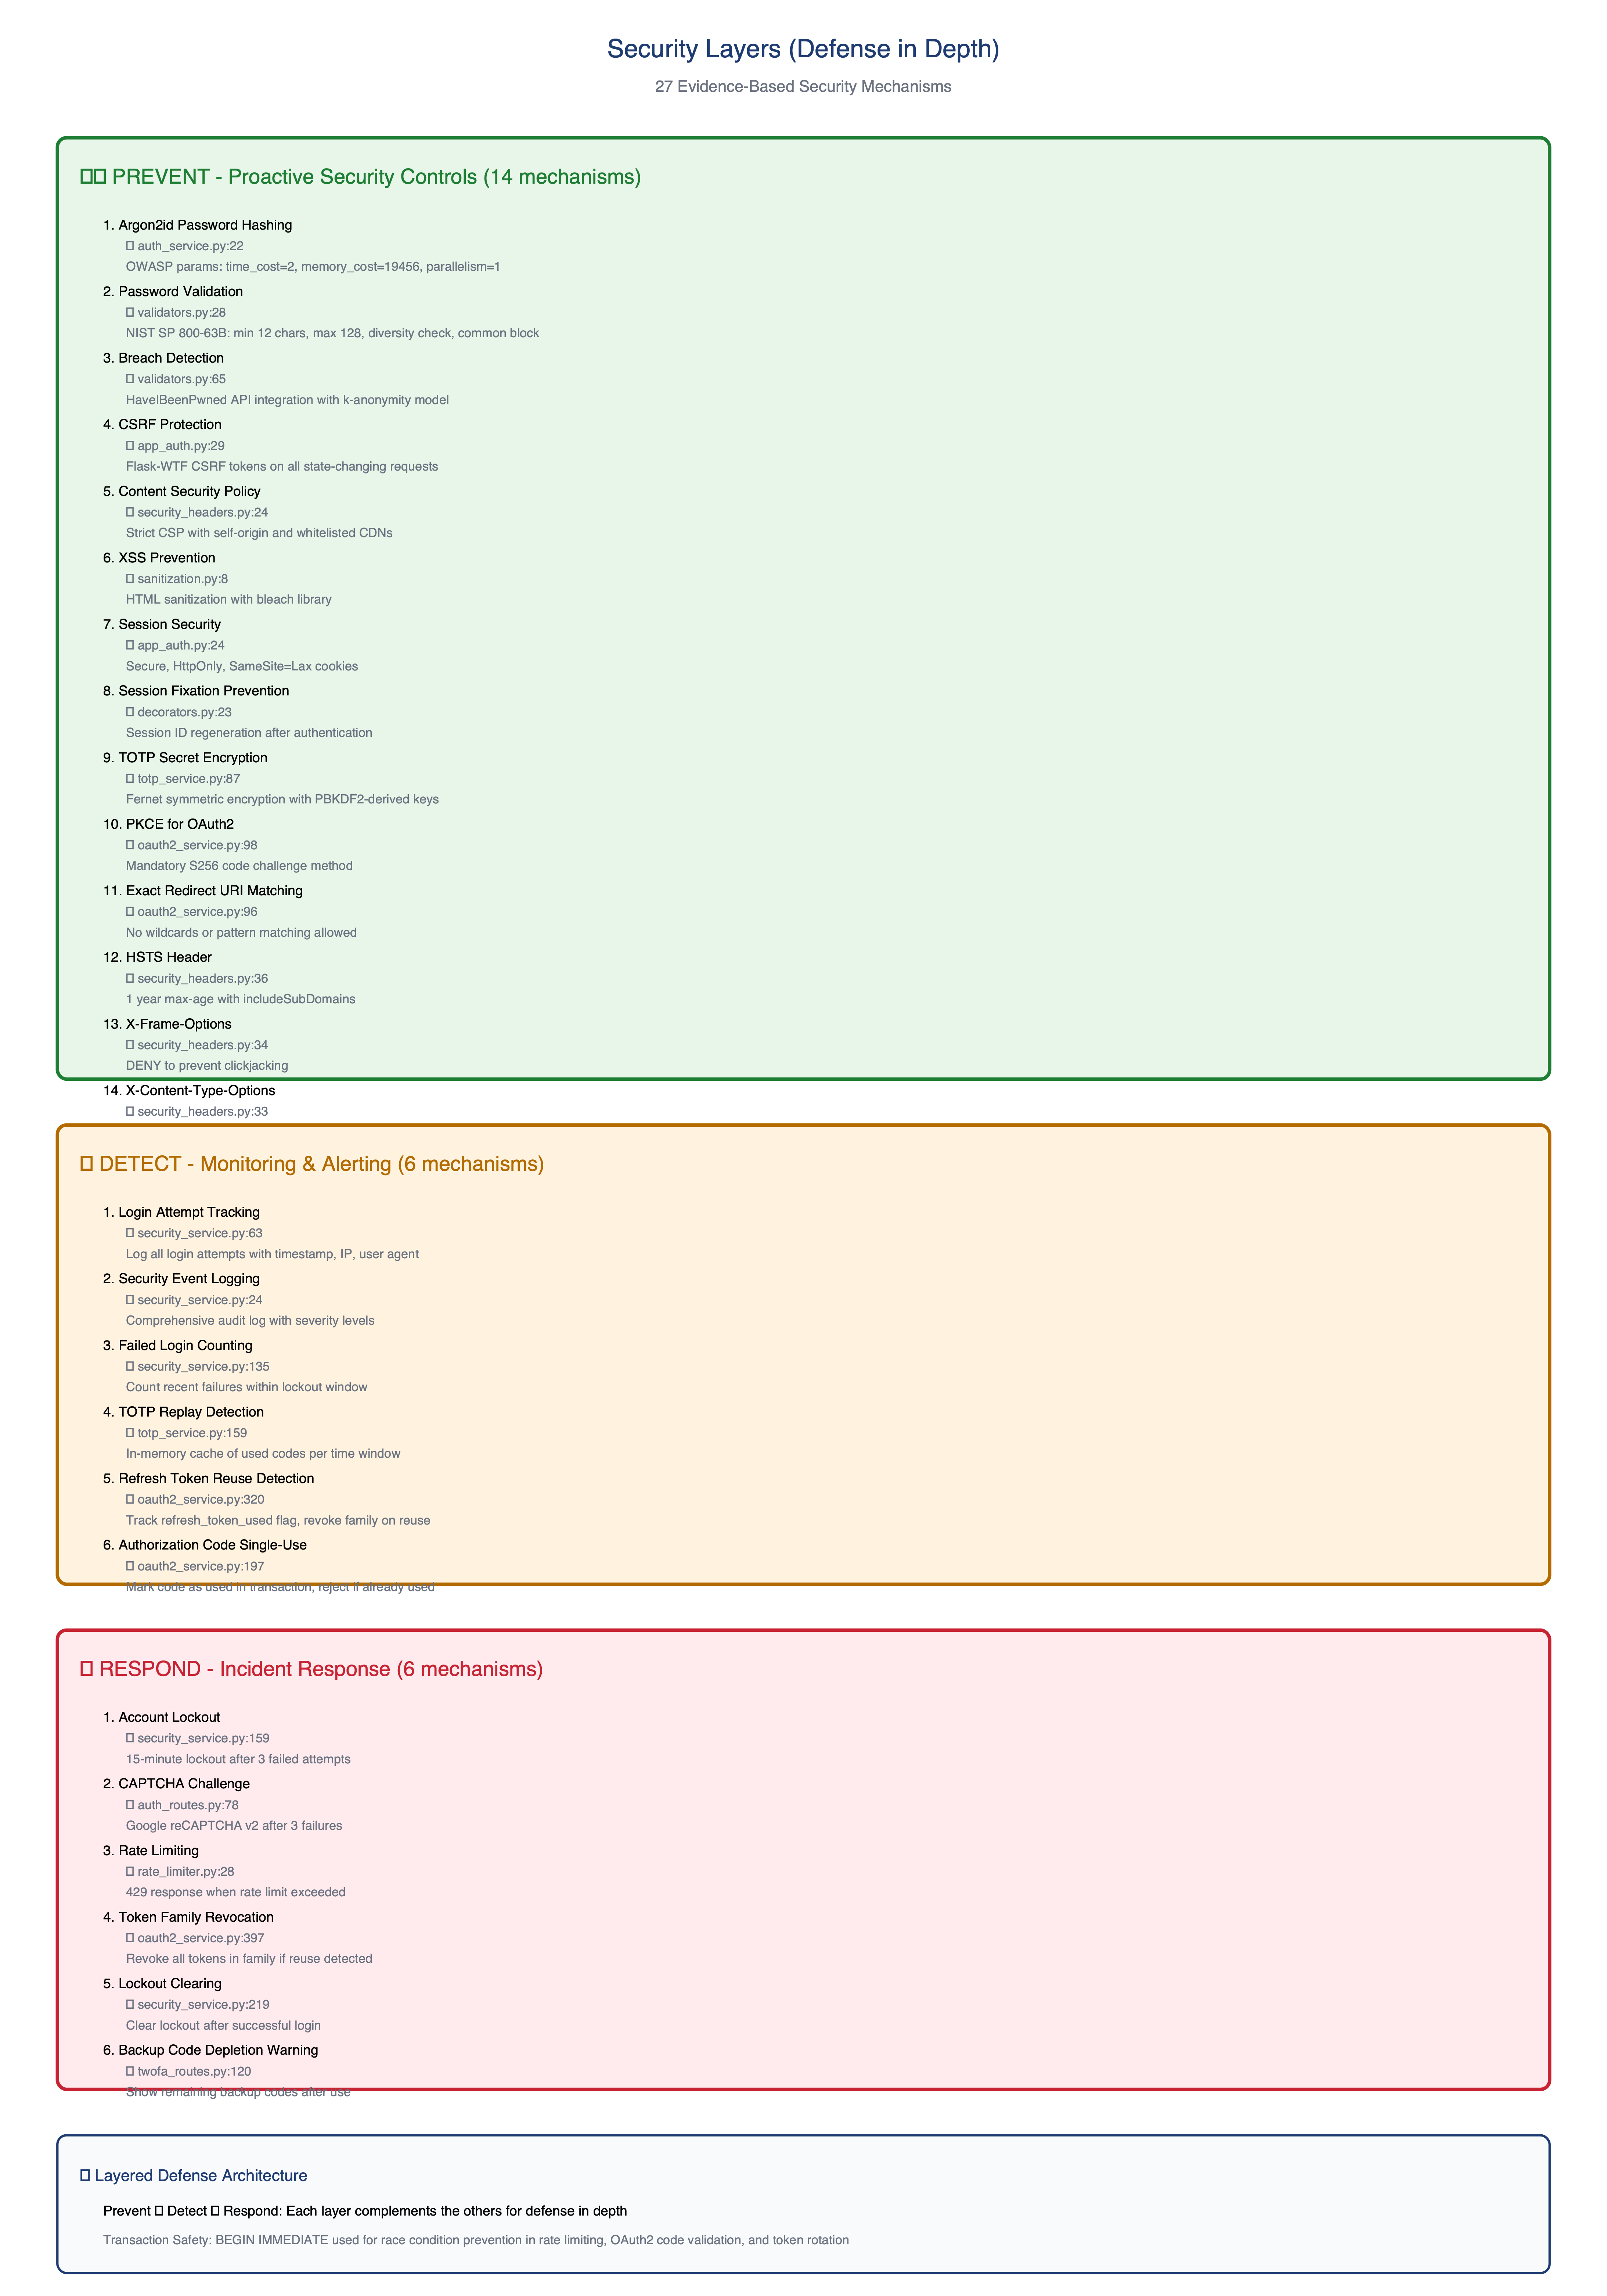
\includegraphics[width=\textwidth]{diagrams/7_security_layers.png}
    \caption{Defense-in-depth architecture with 27 security mechanisms}
    \label{fig:security_layers}
\end{figure}

The architecture includes 14 preventive controls (Argon2id, PKCE, CSRF, CSP, encryption), 6 detective controls (login tracking, security logging, replay detection, reuse detection), and 6 response controls (lockout, CAPTCHA, rate limiting, token revocation).

\subsection{Service Layer Design}

Figure \ref{fig:classes} shows our service layer implementing the Singleton pattern for lifecycle management.

\begin{figure}[H]
    \centering
    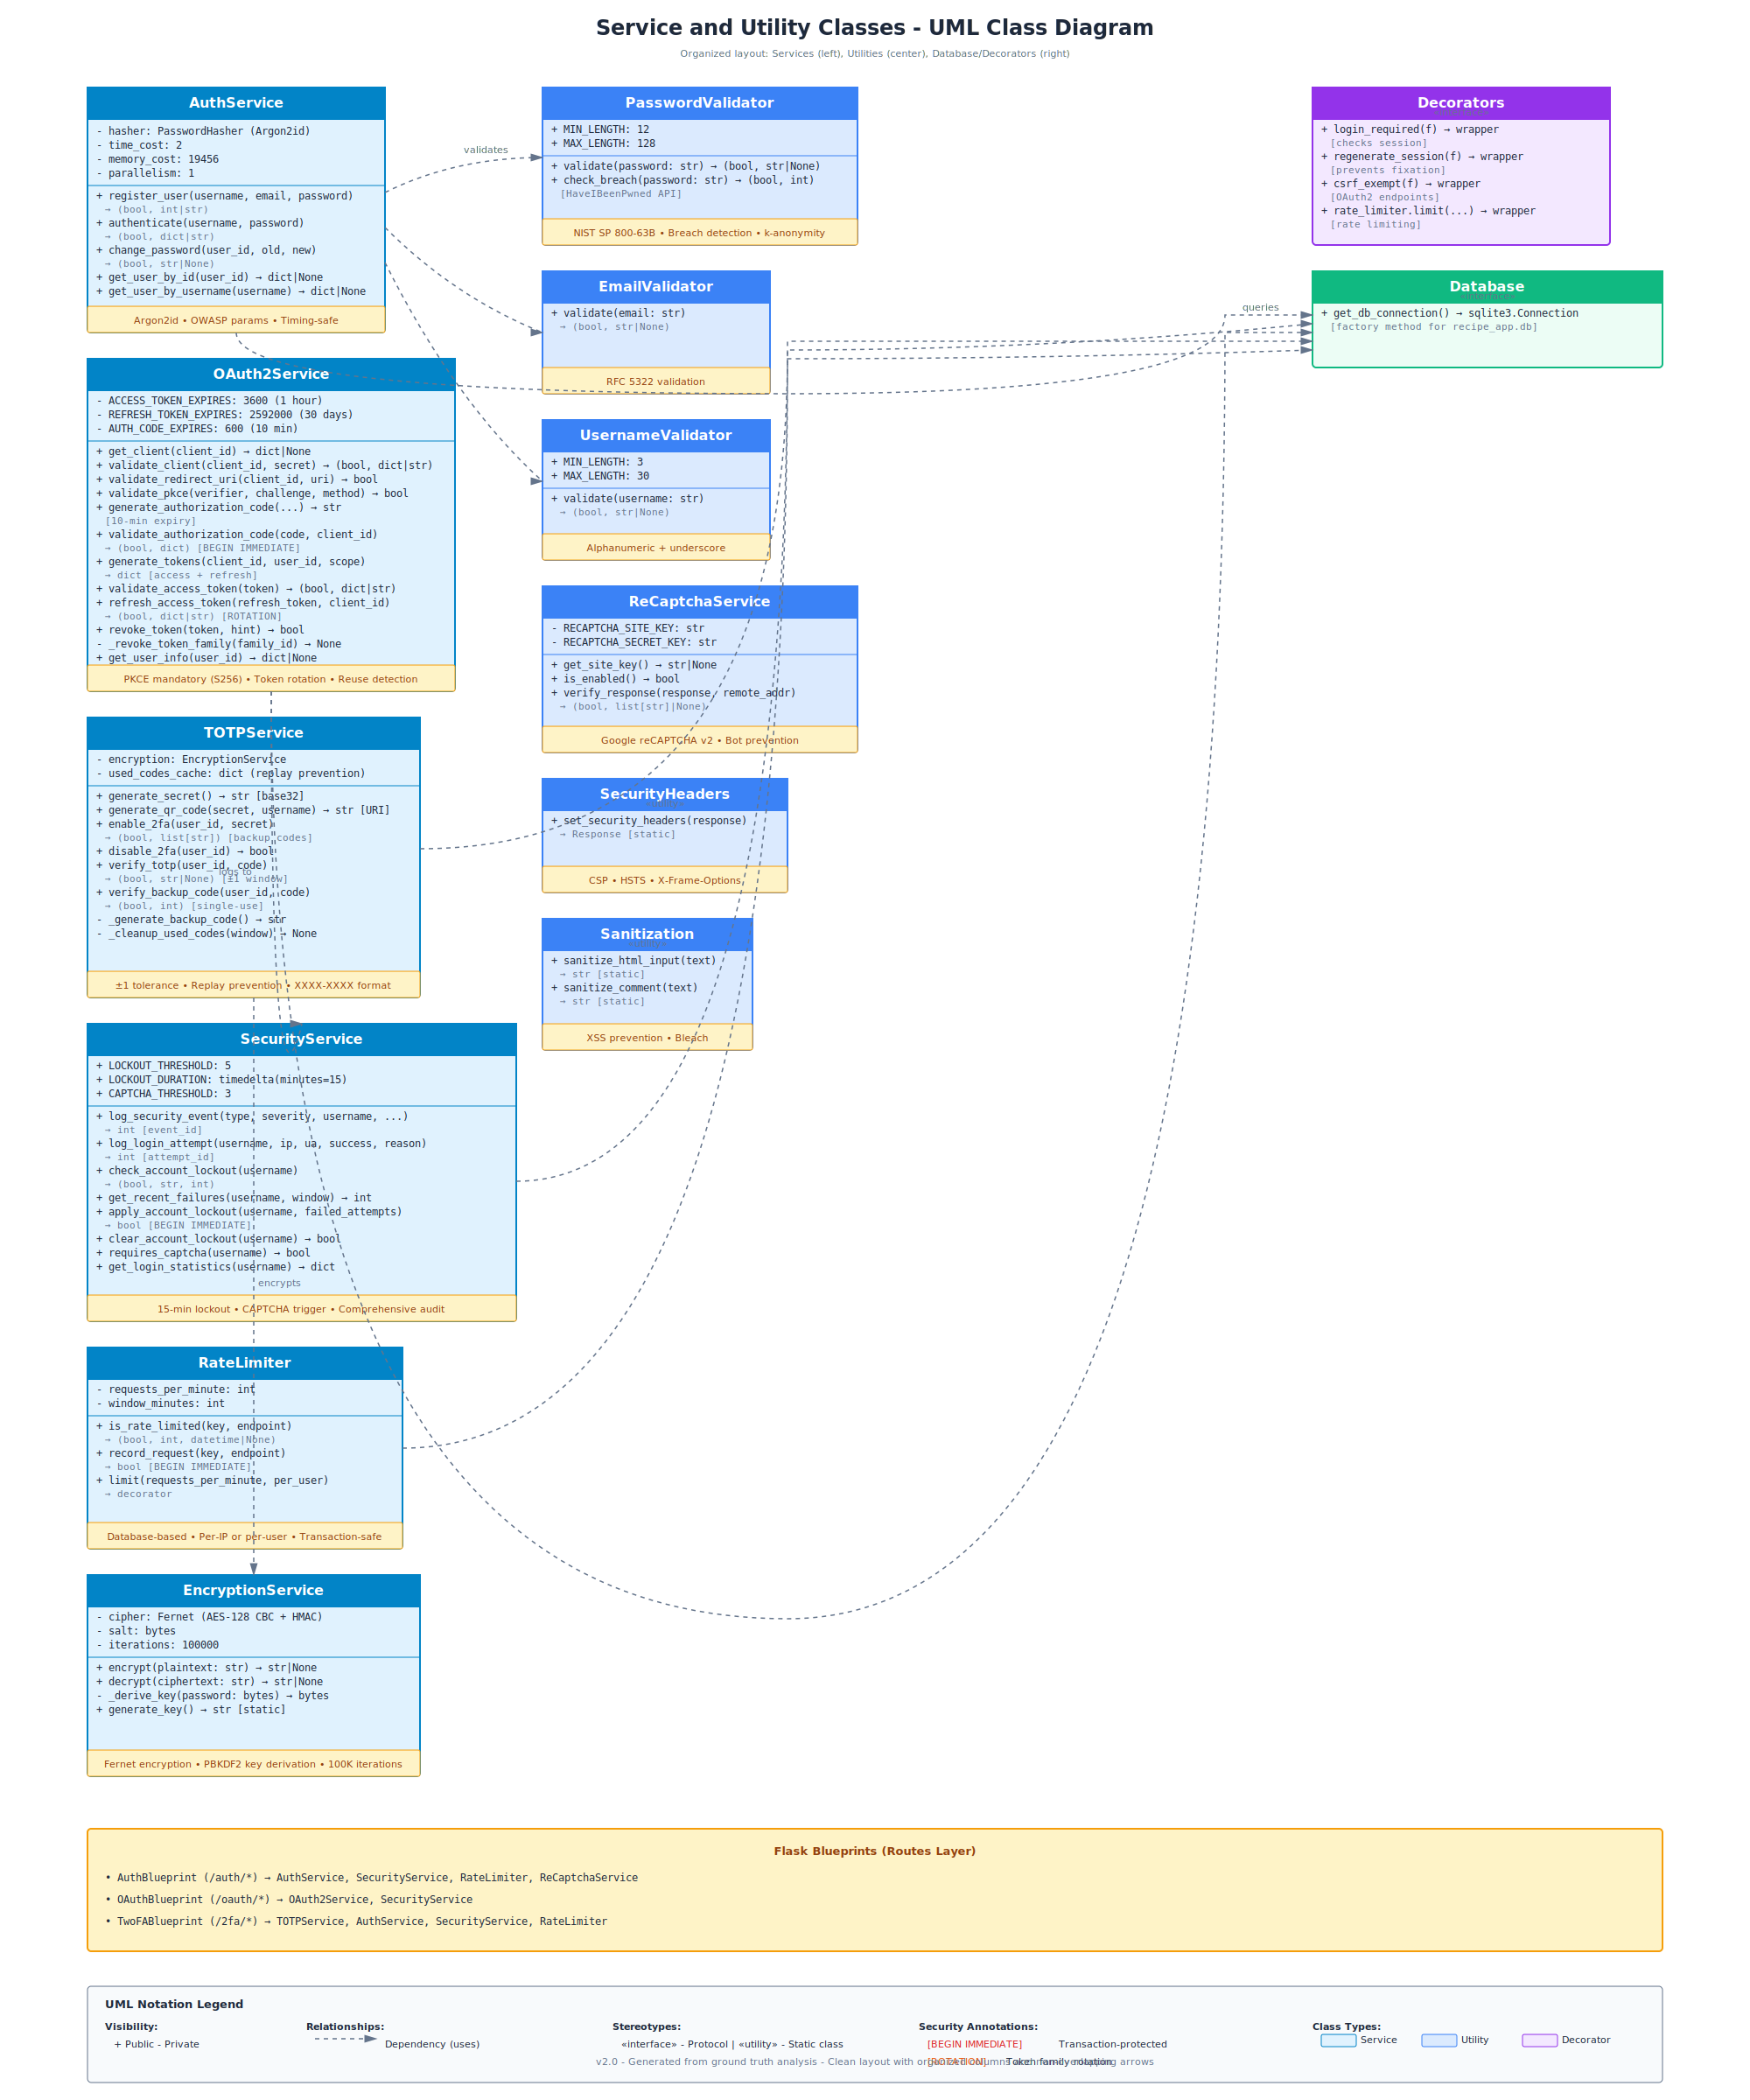
\includegraphics[width=\textwidth]{diagrams/2_class_diagram_services.png}
    \caption{Service layer class diagram with dependencies}
    \label{fig:classes}
\end{figure}

Each service has a single global instance: AuthService (Argon2id hashing), OAuth2Service (PKCE, token rotation), TOTPService (2FA, QR codes), SecurityService (logging, lockout), RateLimiter (database-backed), and EncryptionService (Fernet encryption).

\section{Reflection}

\subsection{Implementation Challenges}

\textbf{Transaction Safety}: SQLite's default \texttt{BEGIN DEFERRED} caused race conditions during concurrent token refreshes. We discovered this through testing and solved it with \texttt{BEGIN IMMEDIATE} transactions at critical locations.

\textbf{Session Fixation}: We initially missed the second session regeneration point after 2FA verification. Testing revealed that sessions needed regeneration at both password authentication and 2FA completion.

\textbf{TOTP Replay Prevention}: Our first implementation didn't prevent code reuse within the same 30-second window. We added an in-memory cache that tracks used codes per time window.

\subsection{Design Decisions}

\textbf{Why Argon2id over bcrypt?} Argon2id is the current OWASP recommendation, memory-hard (prevents GPU attacks), and won the Password Hashing Competition.

\textbf{Why Database-Backed Rate Limiting?} In-memory solutions fail in multi-process deployments (Gunicorn, uWSGI). Database ensures consistent limits across all workers.

\textbf{Why Mandatory PKCE?} OAuth 2.1 draft makes PKCE mandatory for all clients. Provides defense-in-depth even for confidential clients.

\subsection{Real-World Lessons}

Authentication is harder than it looks. Simple mistakes like missing a session regeneration point or using wrong transaction types can create serious vulnerabilities. Following established standards (RFC 6238 for TOTP, RFC 7636 for PKCE, OWASP guidelines) prevented many subtle vulnerabilities we wouldn't have anticipated.

The defense-in-depth approach proved its value. When we accidentally left a timing-attack vulnerability in early testing, the rate limiting and account lockout still prevented exploitation. No single layer is perfect, but together they provide robust security.

\section{Conclusion}

We successfully implemented a production-quality authentication system combining OAuth2 Authorization Code Flow with PKCE, Argon2id password hashing, HIBP breach detection, three-layer brute force protection, and TOTP-based 2FA with replay prevention.

The system implements 27 security mechanisms organized into prevent, detect, and respond categories. All components follow industry best practices (OWASP, RFC standards) and were tested against attack vectors. The comprehensive UML diagrams provide complete documentation with file:line references for maintainability and security audits.

\begin{thebibliography}{9}

\bibitem{owasp}
OWASP Foundation.
\textit{Authentication Cheat Sheet}.
\url{https://cheatsheetseries.owasp.org/}, 2023.

\bibitem{rfc6238}
M'Raihi, D. et al.
\textit{RFC 6238: TOTP Algorithm}.
IETF, 2011.

\bibitem{rfc7636}
Sakimura, N. et al.
\textit{RFC 7636: PKCE for OAuth}.
IETF, 2015.

\bibitem{argon2}
Biryukov, A. et al.
\textit{Argon2: Memory-Hard Password Hashing}.
Password Hashing Competition, 2015.

\end{thebibliography}

\listoffigures

\end{document}
